\documentclass[11pt]{article}
\usepackage[margin=1in]{geometry}
\usepackage{amsmath,amssymb,amsthm,mathtools}
\usepackage{lmodern}
\usepackage[T1]{fontenc}
\usepackage{microtype}
\usepackage{graphicx}
\usepackage{booktabs}
\usepackage{xcolor}
\usepackage[colorlinks=true,linkcolor=blue!50!black,citecolor=blue!50!black,urlcolor=blue!50!black]{hyperref}
\usepackage{cleveref}
\usepackage[section]{placeins}

\newtheorem{proposition}{Proposition}
\newtheorem{remark}{Remark}
\newcommand{\R}{\mathbb{R}}
\newcommand{\N}{N_r}
\newcommand{\code}[1]{\texttt{#1}}
\newcommand{\abs}[1]{\left|#1\right|}
\DeclareMathOperator{\sgn}{sgn}

\title{\texttt{svierosion}: a level set implementation of\\ spherical-volume-invariant erosion flows\\[4pt]
\large Implementation report}
\author{Prepared for J.\ Calder by Claude (Anthropic)}
\date{October 21, 2026}

\begin{document}
\maketitle

\begin{abstract}
This report documents the Python package \code{svierosion} written for the SVI erosion project. The
package erodes a triangulated solid, given as a \code{.ply} file, by the flows with inward normal
velocity $V=\N^k/(t-\N)^s$, where $\N$ is the normalised exterior spherical volume invariant, and by
mean- and Gauss-curvature flows for comparison; it stops at a prescribed fraction of the initial volume
and writes triangulated \code{.ply} meshes. The surface is represented by a signed distance function
on a uniform grid and evolved with a narrow-band level set method: an exact mesh-to-distance
conversion, $\N$ computed for the whole grid by an FFT convolution of exact tangent-plane cell volume
fractions with exact ball/cell overlap weights and evaluated at closest points by tricubic
interpolation, a WENO5/Godunov discretisation, third-order Runge--Kutta time stepping with the nonlocal
velocity recomputed at every stage, subcell-accurate reinitialisation, and step-size control derived from
a linearisation of the flow. All kernels are written in PyTorch and compiled, so the code runs on a GPU
or a CPU. $\N$ is computed with maximal error $10^{-4}$ when the ball radius is $8$ grid cells and
$4\cdot10^{-6}$ at $32$ cells, the flows converge to exact solutions on spheres, and eroding a
$0.8$-million-triangle synthetic scan to $90\%$ of its volume (mesh in, mesh out) takes $9$\,s on a
laptop GPU with $15$M grid nodes and $27$\,s with $50$M nodes ($19$--$29$\,s on 16 CPU cores at
$7$--$15$M nodes).
\end{abstract}

\tableofcontents

%======================================================================
\section{Overview}
%======================================================================

\paragraph{What was built.} The repository contains
\begin{itemize}
\item the package \code{svierosion/} (about 3400 lines; module list in \cref{tab:modules}),
\item a command line interface (\code{python -m svierosion} with subcommands \code{erode},
\code{compare}, \code{distance}, \code{shapes}, \code{info}),
\item toy examples (\code{examples/toy\_examples.py}), accuracy and timing studies
  (\code{benchmarks/}), unit tests (\code{tests/}, 19 tests, run on GPU and CPU),
\item this report (\code{report/}).
\end{itemize}
A typical call is
\begin{verbatim}
python -m svierosion erode fragment.ply -o eroded.ply --radius 2.0 \
       -k 1 -s 1 -t 0.93 --target 0.9 --resolution 400 --snapshots 0.97 0.94
\end{verbatim}
which writes \code{eroded.ply} (and meshes at $97\%$ and $94\%$ of the volume) with per-vertex fields
\code{depth} (distance to the original surface), \code{N} ($\N$ on the eroded surface), \code{speed},
and \code{quality} (a copy of \code{depth} that MeshLab colours), plus a JSON file with parameters and
timings and a CSV file with the time-step history.

\begin{table}[t]
\centering\small
\begin{tabular}{lp{0.6\textwidth}}
\toprule
module & content\\
\midrule
\code{meshio.py} & PLY reader/writer (ascii and binary, any vertex properties), \code{TriMesh}\\
\code{sdf.py} & exact signed distance of a triangle mesh on a grid (\cref{sec:sdf})\\
\code{levelset.py}, \code{kernels.py} & narrow band, WENO5/Godunov, curvatures, cell fractions,
interpolation, reinitialisation\\
\code{svi.py} & ball/cell overlap weights, FFT evaluation of $\N$ (\cref{sec:svi})\\
\code{flows.py} & the speed laws (\cref{sec:model})\\
\code{evolve.py} & time integration and step-size control (\cref{sec:time})\\
\code{surface.py} & marching cubes and projection onto the zero level set\\
\code{api.py}, \code{cli.py}, \code{compare.py} & high-level interface, command line, flow comparisons\\
\code{shapes.py}, \code{viz.py}, \code{figures.py} & test solids, rendering, figures\\
\bottomrule
\end{tabular}
\caption{Package layout.}\label{tab:modules}
\end{table}

\paragraph{Design decisions in brief.}
\begin{enumerate}
\item The solid $\Omega(t)$ is the sublevel set $\{\phi<0\}$ of a signed distance function $\phi$ on a
uniform grid of spacing $h$; only a band $|\phi|<6h$ is evolved. Topological changes (splitting of thin
parts, closing of cavities) are handled automatically.
\item The initial $\phi$ is the \emph{exact} signed distance to the input mesh in the band (to float32
round-off), not a redistanced binary voxelisation.
\item $\N$ is computed on the whole grid at once by one FFT convolution per evaluation, which is cheap
($0.05$\,s for $512^3$ on the GPU), and evaluated at the closest point on the interface of each band node.
The discretisation (tangent-plane cell fractions, exact ball weights, tricubic interpolation) was chosen
after comparing alternatives (\cref{tab:N}); its error is $O(h^2)$ and unbiased.
\item The nonlocal velocity is recomputed at every Runge--Kutta stage. The time step obeys a CFL condition
and an additional restriction coming from the nonlocal feedback, which matters for the singular laws
($s=1$).
\item Everything runs in PyTorch on GPU or CPU; the stencil kernels are fused with \code{torch.compile}
(5--25$\times$ faster than eager PyTorch).
\end{enumerate}

%======================================================================
\section{The flows}\label{sec:model}
%======================================================================

\subsection{The normalised exterior spherical volume invariant}

For a solid $\Omega\subset\R^3$, $x\in\R^3$ and $r>0$ let
\begin{equation}\label{eq:N}
\N(x)=\frac{|B_r(x)\setminus\Omega|}{|B_r|},\qquad |B_r|=\tfrac43\pi r^3 .
\end{equation}
(The instructions say ``divided by $\tfrac43\pi$''; I assumed the intended normalisation is by
$|B_r|=\tfrac43\pi r^3$, so that $\N\in[0,1]$ as stated there.) On the boundary, $\N=\tfrac12$ at flat
points, $\N=1-\theta/2\pi$ on a straight edge of interior dihedral angle $\theta$ (so $3/4$ on a right
angle, $5/6$ on a $60^\circ$ edge, $1/4$ on a re-entrant right angle), $7/8$ at a cube corner and $11/12$
at a corner of an equilateral triangular prism (as long as $r$ is smaller than the distance to other
features). For a ball of radius $R\ge r/2$ the exact value follows from the volume of a lens,
\begin{equation}\label{eq:Nsphere}
\N = 1-\frac{\pi r^2(8Rr-3r^2)/(12R)}{\frac43\pi r^3}=\frac12+\frac{3r}{16R},
\end{equation}
and in general, for a smooth surface \cite{pottmann07},
\begin{equation}\label{eq:Nexp}
\N(x)=\frac12+\frac{3}{16}\,H(x)\,r+O(r^2),\qquad H=\tfrac12(\kappa_1+\kappa_2).
\end{equation}
\Cref{fig:exposure} shows $\N$ on a few test surfaces; for a rough surface it depends strongly on $r$:
with $r$ large the roughness is averaged out and only the large-scale exposure (break edges, outer versus
inner surface) remains.

\begin{figure}[t]
\centering
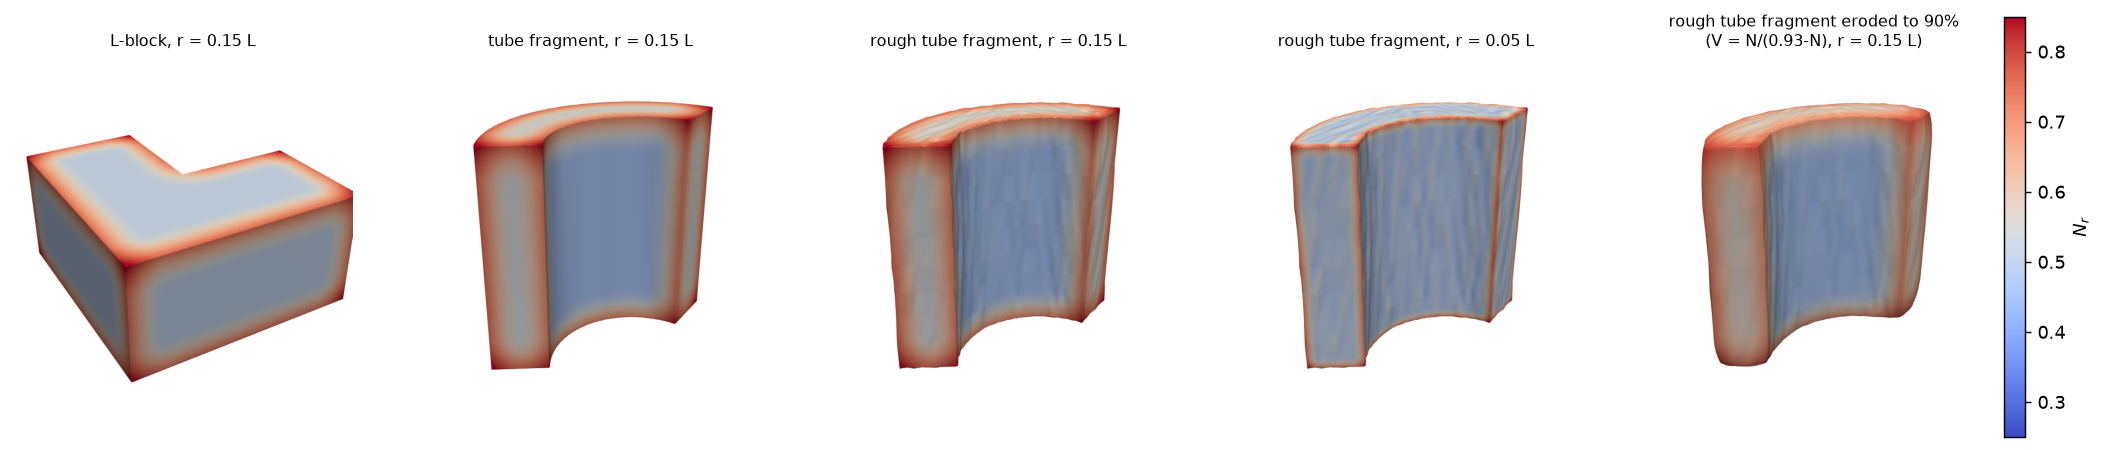
\includegraphics[width=\textwidth]{figures/exposure_maps.png}
\caption{Exposure maps: $\N$ on the surface (blue: $\N<\frac12$, sheltered; red: $\N>\frac12$,
exposed). The rough tube fragment is a synthetic ``scan'' (\cref{sec:perf}); the last panel is the same
object after erosion to $90\%$ volume with $V=\N/(0.93-\N)$.}\label{fig:exposure}
\end{figure}
\begin{remark}
The draft paper (\S2.1) writes $\N=\frac12+CHr+O(r^2)$ with $C=3/8$. With the normalisation by
$|B_r|$ and $H$ the average of the principal curvatures the constant is $3/16$ (it is $3/32$ if $H$
denotes $\kappa_1+\kappa_2$); $3/8$ would correspond to normalising by the volume of a half ball, in which
case the leading term would be $1$ rather than $\frac12$.
\end{remark}

\subsection{The SVI family}

The inward normal velocity is
\begin{equation}\label{eq:law}
V=F(\N),\qquad F(n)=\frac{n^k}{(t-n)^s}\;(+\varepsilon),\qquad k\in\{0,1,2,\dots\},\ s\in\{0,1\},
\end{equation}
with $\frac12<t<1$ when $s=1$. The optional constant $\varepsilon\ge0$ (default $0$) reproduces the
draft's $F(s)=s+\varepsilon$ (with $k=1$, $s=0$, up to the normalisation of time). For $s=1$ the factor
$1/(t-n)=\sum_{j\ge0}n^j/t^{j+1}$ is a geometric series in $n$, which presumably explains the name
``geometric term''. \Cref{tab:ratios} shows how strongly the laws favour exposed points.

\begin{table}[h]
\centering\small
\begin{tabular}{lcccc}
\toprule
law & flat ($\N=\frac12$) & $90^\circ$ edge ($\frac34$) & cube corner ($\frac78$) & re-entrant edge ($\frac14$)\\
\midrule
$k=0$, $s=0$ (grassfire) & 1 & 1 & 1 & 1\\
$k=1$, $s=0$ & 1 & 1.5 & 1.75 & 0.5\\
$k=4$, $s=0$ & 1 & 5.06 & 9.38 & 0.0625\\
$k=0$, $s=1$, $t=0.93$ & 1 & 2.39 & 7.82 & 0.63\\
$k=1$, $s=1$, $t=0.93$ & 1 & 3.58 & 13.7 & 0.32\\
\bottomrule
\end{tabular}
\caption{Speed relative to a flat surface, $F(\N)/F(\frac12)$, at typical features.}\label{tab:ratios}
\end{table}

\paragraph{The constraint $t>\N$.} The law is only defined where $\N<t$. The code computes $\max\N$ on the
initial surface and stops with an explanatory error if it is $\ge t$ (for a cube $\max\N=7/8$, for the
triangular prism $11/12$). During the evolution $\N$ can increase: a plate thinner than $2r$ eroded from
both sides has $\N\to1$ on its faces. Where $\N$ approaches $t$ the speed and the time step degenerate,
so for $s=1$ the code caps $\N$ at the value $n_{\rm cap}<t$ at which $F(n_{\rm cap})=100\,F(\frac12)$
(parameter \code{max\_speed\_ratio}); the number of capped interface nodes is reported at each step.
Physically the cap only means that material with $\N\approx t$ is removed at $100$ times the flat-surface
rate instead of ``instantaneously''. In the toy examples of \cref{sec:toy} ($t=0.93$) the cap was never
active: the largest initial value, $\N=0.915$ at the prism corners, is below $n_{\rm cap}=0.922$ ($k=1$);
with $t=0.92$ it acted on a handful of corner nodes during the first step.

\subsection{Level set formulation}

Let $\phi(\cdot,t)$ be negative in $\Omega(t)$ and positive outside. A boundary moving with inward normal
speed $V\ge0$ satisfies
\begin{equation}\label{eq:ls}
\phi_t = V\,|\nabla\phi| .
\end{equation}
(Indeed, for $\phi=x_1-a(t)$ the boundary moves inwards iff $a'<0$ iff $\phi_t>0$.)
\begin{remark}
Equations (6.1) and (6.2) of the draft use $u_t=-Q|\nabla u|$ with $u<0$ inside; with that sign the
object grows. The student's code uses the correct sign.
\end{remark}
Because $V(x)=F(\N(x;\Omega(t)))$ depends on the whole set, \eqref{eq:ls} is a nonlocal
Hamilton--Jacobi equation of the type studied by Slep\v{c}ev \cite{slepcev03}. The flow is
order preserving: if $\Omega_1\subset\Omega_2$ touch at $x$, then $B_r(x)\setminus\Omega_1\supset
B_r(x)\setminus\Omega_2$, so $\N(x;\Omega_1)\ge\N(x;\Omega_2)$ and, $F$ being nondecreasing,
$\Omega_1$ erodes at least as fast as $\Omega_2$ at $x$. This monotonicity is the structural hypothesis
for a comparison principle and a viscosity-solution theory in that framework; I have not checked the
remaining (continuity) hypotheses, which are delicate for $s=1$ near $\N=t$.
Off the interface, the velocity is defined by \emph{extension constant along normals}:
\begin{equation}\label{eq:ext}
V(x)=F\big(\N(\pi(x))\big),\qquad \pi(x)=x-\phi(x)\frac{\nabla\phi(x)}{|\nabla\phi(x)|^2},
\end{equation}
($\pi$ is the closest point projection when $\phi$ is a signed distance function). With this extension
$|\nabla\phi|=1$ is preserved by the exact flow, which keeps $\phi$ close to a distance function between
reinitialisations. (The alternative, evaluating $\N$ at every node, moves each level set with its own
invariant; it is also consistent, but it distorts $\phi$ and, as \cref{tab:N} shows, nodal values of $\N$
differ from interface values by $O(h/r)$.)

\subsection{Linearisation and what it implies}\label{sec:linear}

Perturb a plane: $\Omega=\{z<\delta\cos(\xi\cdot y)\}$, $y\in\R^2$, $\xi\in\R^2$. Expanding the exterior
volume of the ball centred at a boundary point to first order in $\delta$ gives
\begin{equation}\label{eq:symbol}
\N = \frac12+\frac{3}{4r}\,\delta\cos(\xi\cdot y)\Big(1-\frac{2J_1(|\xi| r)}{|\xi| r}\Big)+O(\delta^2).
\end{equation}
For $|\xi|r\ll1$, $1-2J_1(z)/z\approx z^2/8$ and \eqref{eq:symbol} reduces to \eqref{eq:Nexp} (the
mean curvature of the graph is $\frac12|\xi|^2\delta\cos$). Linearising \eqref{eq:ls}, a mode decays at
the rate
\begin{equation}\label{eq:rate}
\lambda(\xi)=F'(\tfrac12)\,\frac{3}{4r}\Big(1-\frac{2J_1(|\xi| r)}{|\xi| r}\Big)\ \le\ 1.132\cdot F'(\tfrac12)\,\frac{3}{4r},
\end{equation}
since $\max_z(1-2J_1(z)/z)\approx1.132$ (attained at $z\approx5.14$). Three consequences:
\begin{enumerate}
\item The SVI flow is \emph{not} parabolic: at wavelengths below $r$ it acts like a zeroth-order operator
and damps all of them at the same finite rate $\approx F'\cdot3/(4r)$. A convex corner or edge is a shock
of \eqref{eq:ls} (characteristics collide) and stays a kink; it only opens up gradually, at a rate set by
the gradient of $V$ along the adjacent faces. This is visible in all examples (\cref{sec:toy}) and is in
sharp contrast with curvature flows, which round corners instantly. Likewise, surface roughness at scales
$\ll r$ is removed at the rate $\approx F'(\N)\cdot3/(4r)$, i.e. slowly when $r$ is large.
\item The large-scale behaviour is grassfire with speed $F(\frac12)$ plus a mean-curvature-like correction
of relative weight $\frac{3r}{16}F'(\frac12)/F(\frac12)$; for $F=n^k/(t-n)^s$ this weight is
$\frac{3r}{16}\,(2k+\frac{s}{t-1/2})$. This matches the observation in the draft that larger $k$ gives
more smoothing; the geometric term adds the equivalent of $k\approx 1/(2(t-\frac12))$ at large scales, but
acts much more strongly at exposed features (\cref{tab:ratios}), where it is nonlinear.
\item An explicit time step must resolve the relaxation rate \eqref{eq:rate} evaluated at the current
$\N$, which is large near exposed points when $s=1$ (\cref{sec:time}).
\end{enumerate}

\subsection{Comparison flows: curvature laws}\label{sec:curvlaws}

The comparison flows are
\begin{equation}\label{eq:curvlaws}
V=(H_+)^\alpha\quad\text{(mean)},\qquad V=\big((\kappa_1)_+(\kappa_2)_+\big)^\alpha\quad\text{(Gauss)},
\end{equation}
with $\kappa_i=1/R$ on a sphere of radius $R$. The Gauss law equals the Gauss curvature $K$ at convex
points and $0$ elsewhere. I deliberately did \emph{not} use $K_+=\max(K,0)$: $K>0$ also at concave
elliptic points (the bottom of a pit), where $\partial K/\partial\kappa_i<0$ and the flow $V=K$ is backward
parabolic; eroding a pit faster the more concave it is is also non-physical. Both laws in
\eqref{eq:curvlaws} are nondecreasing functions of the principal curvatures, hence degenerate parabolic,
so the level set equation is well posed in the viscosity sense \cite{evansspruck}. $\alpha=1/4$ gives the
affine-invariant flow of Rayleigh and Andrews, $\alpha=1$ Firey's model.

For $\alpha<1$, $x\mapsto x^\alpha$ has infinite slope at $0$, which makes the parabolic time step of an
explicit scheme collapse ($\Delta t\to0$ was observed). The code therefore uses
\begin{equation}
x^\alpha \approx x\,(x+\delta)^{\alpha-1},
\end{equation}
which equals $x^\alpha(1+O(\delta/x))$ for $x\gg\delta$, is linear with slope $\delta^{\alpha-1}$ near $0$,
and (unlike $(x+\delta)^\alpha-\delta^\alpha$) has no constant offset. The default is $\delta=1/L$ for $H$
and $\delta=1/L^2$ for $K$ ($L$ = largest extent of the object): radii of curvature $\gtrsim L$ are treated
as flat; for $V=K^{1/4}$ the speed changes by $6\%$ at curvature radius $0.3L$ and by $0.7\%$ at
$0.1L$.

The Gauss laws are stiff on solids with sharp edges: at an edge with $\kappa_1\sim1/h$ and $\kappa_2=0$,
$\partial V/\partial\kappa_2=F'(K)\kappa_1\sim F'(0)/h$, so bending perturbations \emph{along} the edge are
diffused with coefficient $\sim F'(0)/h$ and an explicit step needs $\Delta t\lesssim h^3/F'(0)$. This is a
property of Gauss curvature flow, not of the discretisation: removing the parabolic restriction produced
$|H|\sim10^6$ within a few hundred steps. On the unit cube at $96$ cells, $V=K_+$ needs $5.4\cdot10^3$
steps ($30$\,s) to reach $90\%$ volume, while $V=K_+^{1/4}$ had removed less than $1\%$ of the volume
after $2\cdot10^4$ steps, because only the corners move and the edges stay sharp. A semi-implicit scheme would be the remedy
(\cref{sec:future}).

%======================================================================
\section{Numerical method}
%======================================================================

\subsection{Grid and narrow band}

The grid has nodes $x_{ijk}=o+h(i,j,k)$; node $(i,j,k)$ also represents the cube cell of side $h$
centred on it. $h$ is either given or set to $L/\text{resolution}$. The grid covers the bounding box of
the input plus a padding of $\max(r+3h,\,12h)$ on each side (the convolution of \cref{sec:svi} is
circular and exact only if the solid stays $r$ away from the boundary), and its dimensions are rounded
up to $2^a3^b5^c7^d$ for fast FFTs. $\phi$ is a dense float32 array; the band $B=\{|\phi|<6h\}$ is stored
as a sorted list of flat indices, and outside it $\phi$ is clamped to $\pm6h$. All stencils are
evaluated by gathering $\phi$ at flat offsets $\pm m\cdot\mathrm{stride}$; band nodes are kept at least
$4$ cells from the boundary so no gather leaves the array.

\subsection{From a triangle mesh to a signed distance function}\label{sec:sdf}

\paragraph{Distance.} Exact distances are computed in three stages, following the idea of Batty's SDFGen
but vectorised.
\begin{enumerate}
\item \emph{Near field.} Triangles longer than $8h$ are midpoint-subdivided (this does not change the
surface). Each triangle is paired with all nodes of its bounding box dilated by $2h$; the exact
point--triangle distance is computed (Ericson's region classification) and the packed $64$-bit key
\[(\text{float bits of the distance})\ll 32\ \big|\ \text{triangle id}\]
is scatter-minimised into the grid. Because non-negative float32 bit patterns are ordered like the
numbers, this yields in one pass the exact distance \emph{and} the closest triangle of every node within
$2h$ of the surface.
\item \emph{Propagation.} The next rings of nodes (up to $6h$) take the minimum distance to the closest
triangles of their 26 neighbours.
\item \emph{Refinement.} Every node beyond the exact zone re-tests all triangles incident to a vertex of
its current closest triangle (two passes). Without this step the error beyond $2h$ was up to $0.07h$ on a
finely tessellated sphere (neighbouring nodes do not always share the closest triangle when triangles are
smaller than $h$); with it the band agrees with brute force to $10^{-5}h$ (\cref{tab:sdf}).
\end{enumerate}

\paragraph{Sign.} The sign is decided for every node by scanline ray casting: each triangle is rasterised
onto the grid lines parallel to the $x$-axis that pierce it, and the crossing abscissae are accumulated
with a cumulative sum along the lines. The point-in-triangle test is done in float64 with
Simulation-of-Simplicity tie-breaking (the orientation predicate is antisymmetric, including in the
degenerate case), so a grid line through a shared edge or vertex is counted exactly once; this matters for
toy solids whose faces lie exactly on grid planes. For consistently oriented meshes the signed crossing
count (winding number) is used, otherwise the parity; for meshes with holes or non-manifold edges a
majority vote over the three axis directions is taken. The cost is linear in the number of triangles plus
grid lines.

\begin{table}[h]
\centering\small
\begin{tabular}{llccc}
\toprule
mesh & grid & $\max|\phi-d|/h$ & sign errors & time [s] \\
\midrule
cube (12 tri) & 35x35x35 & $3.5\cdot 10^{-7}$ & 0 & 0.35 \\
cube (12 tri) & 81x81x81 & $4.9\cdot 10^{-7}$ & 0 & 0.06 \\
cube (12 tri) & 162x162x162 & $4.9\cdot 10^{-7}$ & 0 & 0.16 \\
torus (36864 tri), 20k band nodes & 108x108x48 & $9.9\cdot 10^{-6}$ & -- & 0.14 \\
torus (36864 tri), 20k band nodes & 216x216x96 & $2.1\cdot 10^{-5}$ & -- & 0.39 \\
\bottomrule
\end{tabular}

\caption{Signed distance accuracy: exact distance $d$ (analytic for the cube; brute force over all
triangles for $2\cdot10^4$ random band nodes of the torus).}\label{tab:sdf}
\end{table}

\subsection{Cell volume fractions}\label{sec:fractions}

The occupancy of the cell $C$ of node $c$ is approximated by the exact volume fraction of $C$ below the
tangent plane of $\phi$,
\begin{equation}
f_c=\frac{|\{\xi\in C:\ \phi(c)+\nabla\phi(c)\cdot(\xi-c)<0\}|}{h^3},
\end{equation}
with $\nabla\phi$ by central differences. Writing $n=\nabla\phi/|\nabla\phi|$, $s=\phi(c)/(h|\nabla\phi|)$
and $U_i$ i.i.d.\ uniform on $[-\frac12,\frac12]$, $f_c=P(\sum_i n_iU_i<-s)$, the distribution function of
a sum of three uniforms. With $a\ge b\ge c\ge0$ the sorted $|n_i|$ and $y=\frac{a+b+c}{2}-s$,
\[
P=\frac{1}{6abc}\sum_{\epsilon\in\{0,1\}^3}(-1)^{|\epsilon|}\big(y-\epsilon\cdot(a,b,c)\big)_+^3,
\]
which is useless in single precision when $b$ or $c$ is small (catastrophic cancellation; axis-aligned
faces have $b=c=0$). Using the symmetry $P(y)=1-P(a+b+c-y)$ it suffices to take $y\le\frac{a+b+c}2$, where
only five terms survive, and they can be grouped without cancellation:
\[
f=\frac{G(y)}{6a}-\frac{(y-a)_+^3}{6abc},\qquad
G(y)=\begin{cases}
y^3/(bc), & y\le c,\\
(3y^2-3cy+c^2)/b, & c<y\le b,\\
\big(3y^2-3cy+c^2-(y-b)^3/c\big)/b, & b<y\le b+c,\\
3(2y-b-c), & y>b+c.
\end{cases}
\]
Each piece is bounded independently of $b,c$ (e.g.\ $(y-b)^3/c\le c^2$ on its interval, and the last term
is non-zero only if $a<b+c$, where it is $\le c^2/(8b)$). The tangent-plane fraction is exact for planes and
has an $O(h^2\kappa)$ error per cut cell. Compared with a smoothed Heaviside $H_\epsilon(\phi)$ it removes
the $O(h^2)$ \emph{bias} of the computed volume invariant (\cref{tab:N}, last row). The volume of the solid
is $h^3\sum_c f_c$; it is used for the stopping criterion.

\subsection{\texorpdfstring{Computing $N_r$}{Computing N\_r}}\label{sec:svi}

\paragraph{Ball weights.} The interior volume at a node is approximated by
\begin{equation}\label{eq:conv}
|B_r(x)\cap\Omega|\approx h^3\sum_y w(x-y)\,f_y,\qquad w(z)=\frac{|B_r(0)\cap C_z|}{h^3},
\end{equation}
which is exact for every cell that is not cut by both $\partial\Omega$ and $\partial B_r(x)$; those
cells form a curve of $O(r/h)$ cells, each contributing $O(h^3)$, which gives a relative error
$O(h^2/r^2)$. The weights $w$ are the exact overlaps of the ball with the cells: cells entirely inside
($w=1$) or outside ($w=0$) are classified exactly; for cut cells the $z$-extent of the ball is integrated
analytically and the remaining 2-d integral over $(x,y)$ by $32\times32$ Gauss--Legendre points. The sum of
the weights equals $|B_r|/h^3$ to $10^{-5}$ relative.

\paragraph{FFT.} \eqref{eq:conv} is a discrete convolution, evaluated with real FFTs (cuFFT on the GPU,
PyTorch's multi-threaded FFT on the CPU). The kernel transform is computed once. Because the solid
stays at least $r$ from the boundary, the circular convolution coincides with the linear one at every node
within $r$ of the solid, so no zero padding is needed. One evaluation costs two FFTs of the grid:
$0.05$\,s for $512^3$ on the laptop GPU and $0.35$\,s on 16 CPU cores.

\paragraph{Evaluation at the interface.} $\N$ at a band node is replaced by $\N(\pi(x))$, see
\eqref{eq:ext}, computed by tricubic (tensor Lagrange) interpolation of the dense $\N$ field. Two remarks
explain why this matters. First, $\N$ varies across the interface at rate $\partial_\nu\N=\frac{3}{4r}$
(from $\N(d)=\frac12+\frac34\frac dr-\frac14\frac{d^3}{r^3}$ for a plane at signed distance $d$), so the
value at the nearest node differs from the interface value by up to $\frac34\cdot\frac{\sqrt3}2\,h/r$,
about $0.08$ for $r=8h$. Second, $\N$ is smooth near the interface ($\partial^2_\nu\N=0$ on a plane), so
tricubic interpolation is very accurate there, whereas trilinear interpolation has an $O(h^2/r^2)$ error
that dominates everything else.

\Cref{tab:N} compares the occupancy models (binary indicator, the sine-smoothed Heaviside of width $h$
used by the student code, tangent-plane fractions) and interpolations on a sphere of radius $1$ with
$r=0.4$ against \eqref{eq:Nsphere}. The ``student-like'' rows reproduce the student code's discretisation
(smoothed Heaviside, ball voxelised with $3^3$ samples per cell and renormalised by its sum, value at the
nodes); since the level set update effectively interpolates nodal speeds linearly, the row with linear
interpolation is the fairer comparison: at $r/h=8$ its error is $8\cdot10^{-4}$, eight times that of the
method used, and the difference is due mostly to the interpolation, not to the ball voxelisation. The row
``nodal'' shows the size of the difference between nodal and interface values, $O(h/r)$.

\begin{table}[h]
\centering\footnotesize\setlength{\tabcolsep}{3.5pt}
\begin{tabular}{lccccccc}
\toprule
method $\backslash$ $r/h$ & $4$ & $6$ & $8$ & $12$ & $16$ & $24$ & $32$ \\
\midrule
planes + tricubic (used) & $6.5\cdot 10^{-4}$ & $2.1\cdot 10^{-4}$ & $9.8\cdot 10^{-5}$ & $5.3\cdot 10^{-5}$ & $3.9\cdot 10^{-5}$ & $9.9\cdot 10^{-6}$ & $3.6\cdot 10^{-6}$ \\
planes + trilinear & $4.3\cdot 10^{-3}$ & $1.8\cdot 10^{-3}$ & $1.0\cdot 10^{-3}$ & $4.6\cdot 10^{-4}$ & $2.6\cdot 10^{-4}$ & $1.1\cdot 10^{-4}$ & $6.3\cdot 10^{-5}$ \\
Heaviside + tricubic & $7.4\cdot 10^{-4}$ & $3.1\cdot 10^{-4}$ & $1.7\cdot 10^{-4}$ & $8.1\cdot 10^{-5}$ & $4.5\cdot 10^{-5}$ & $1.8\cdot 10^{-5}$ & $9.5\cdot 10^{-6}$ \\
Heaviside + trilinear & $3.8\cdot 10^{-3}$ & $1.6\cdot 10^{-3}$ & $9.4\cdot 10^{-4}$ & $4.0\cdot 10^{-4}$ & $2.3\cdot 10^{-4}$ & $1.0\cdot 10^{-4}$ & $5.6\cdot 10^{-5}$ \\
binary + tricubic & $1.8\cdot 10^{-2}$ & $7.9\cdot 10^{-3}$ & $5.2\cdot 10^{-3}$ & $2.6\cdot 10^{-3}$ & $1.4\cdot 10^{-3}$ & $5.1\cdot 10^{-4}$ & $4.0\cdot 10^{-4}$ \\
student-like + trilinear & $3.2\cdot 10^{-3}$ & $1.4\cdot 10^{-3}$ & $8.1\cdot 10^{-4}$ & $3.8\cdot 10^{-4}$ & $2.5\cdot 10^{-4}$ & $1.2\cdot 10^{-4}$ & $5.7\cdot 10^{-5}$ \\
student-like, nodal & $1.4\cdot 10^{-1}$ & $9.0\cdot 10^{-2}$ & $7.3\cdot 10^{-2}$ & $4.6\cdot 10^{-2}$ & $3.7\cdot 10^{-2}$ & $2.4\cdot 10^{-2}$ & $1.8\cdot 10^{-2}$ \\
\midrule
used: mean signed error & $3.0\cdot 10^{-5}$ & $-2.2\cdot 10^{-6}$ & $-2.0\cdot 10^{-6}$ & $-7.0\cdot 10^{-7}$ & $-4.0\cdot 10^{-7}$ & $-4.1\cdot 10^{-7}$ & $-1.8\cdot 10^{-7}$ \\
\bottomrule
\end{tabular}

\caption{Maximal error of $\N$ over $5000$ points of a sphere ($R=1$, $r=0.4$, exact value
$0.575$) as a function of $r/h$. ``planes'': tangent-plane cell fractions; ``Heaviside'': sine-smoothed
Heaviside of half-width $h$; ``binary'': $\mathbf 1_{\phi<0}$; ``student-like'': smoothed Heaviside with
a $3^3$-supersampled ball renormalised by its sum. The used method (first row) has $O(h^2)$ error and
essentially no bias (last row).}
\label{tab:N}
\end{table}

\subsection{Spatial discretisation of the level set equation}

$|\nabla\phi|$ in \eqref{eq:ls} is discretised by the Godunov flux for the concave Hamiltonian
$\mathcal H(p)=-V|p|$, $V\ge0$, applied dimension by dimension. In one dimension, with one-sided
derivatives $p^\pm$, the Godunov flux is $\min_{[p^-,p^+]}\mathcal H$ if $p^-\le p^+$ and
$\max_{[p^+,p^-]}\mathcal H$ otherwise; checking the six sign cases gives
\begin{equation}\label{eq:godunov}
|\nabla\phi|^2\approx\sum_{i=1}^3\max\big(\min(D_i^-\phi,0)^2,\ \max(D_i^+\phi,0)^2\big).
\end{equation}
$D^\pm_i\phi$ are the fifth-order WENO approximations of Jiang and Peng \cite{jiangpeng} from the seven
values $\phi_{i-3},\dots,\phi_{i+3}$ (with $\varepsilon=10^{-6}\max v_j^2+10^{-10}$ in the smoothness
weights; the additive floor must not underflow when squared in float32). The scheme is monotone in the
first-order limit and fifth order in smooth regions. Near the band edge the velocity is multiplied by a
smooth cutoff (equal to $1$ for $|\phi|\le4h$ and to $0$ for $|\phi|\ge5.5h$), as in the local level set
method of Peng et al. \cite{peng}.

\subsection{Time integration and step-size control}\label{sec:time}

The semi-discrete system $\dot\phi=L(\phi)=V(\phi)\,|\nabla\phi|$ is integrated with the three-stage TVD
Runge--Kutta method of Shu and Osher. $V$ depends on $\phi$ nonlocally; it is \emph{recomputed at every
stage} (fractions, FFT, closest points, interpolation), so the coupling is third order in time as well.
The step is
\begin{equation}\label{eq:dt}
\Delta t=\min\Big(\underbrace{0.5\,\frac{h}{\max V}}_{\text{CFL}},\ \underbrace{1.0\cdot\frac{4r/3}{\max_{\partial\Omega}F'(\N)}}_{\text{nonlocal feedback}},\ \underbrace{0.25\,\frac{h^2}{\max(\partial_{\kappa_1}V+\partial_{\kappa_2}V)}}_{\text{curvature laws only}}\Big).
\end{equation}
The second term bounds $\lambda\Delta t\le1.13$ in \eqref{eq:rate}, safely inside the stability interval
$[-2.51,0]$ of the RK3 method and close to the non-oscillation threshold $1$ of forward Euler. It is the
active restriction for the singular laws near exposed points: for $F=n/(t-n)$, $F'/F=1/n+1/(t-n)$, and with
$t-\N=0.02$ and $r=10h$ the CFL step would give $\lambda\Delta t\approx2$.

\paragraph{Stopping at the volume fraction.} After every step the volume $h^3\sum f_c$ is compared with the
target $\theta V_0$. If a step overshoots, it is repeated from the stored state with $\Delta t$ obtained by
regula falsi on $\Delta t\mapsto V(\Delta t)$ (2--3 iterations), so the final volume matches the target to
$10^{-6}$ relative. The volume of the output mesh agrees with the level-set volume to a few
$10^{-5}$ (relative) in the examples.

\subsection{Reinitialisation}

Every time the interface may have moved $1.5$ cells (accumulated $\Delta t\max V$), $\phi$ is reinitialised
on the band dilated by three cells by solving $\phi_\tau+\sgn(\phi^0)(|\nabla\phi|-1)=0$ with the scheme of
Min \cite{min10}: second-order ENO differences, TVD-RK2 in pseudo-time with local steps, and the
\emph{subcell resolution} fix: at a node whose neighbour has the opposite sign, the interface position
along that grid line is computed from a quadratic ENO interpolant of $\phi^0$, and the one-sided
difference towards it uses $\phi=0$ at that position. This anchors the zero level set to second order.
After $40$ iterations starting from a strongly distorted function the interface moved by at most
$0.006h$ and the volume by $O(h^2)$ (\cref{tab:reinit}). The band is rebuilt after each reinitialisation.

\begin{table}[h]
\centering\small
\begin{tabular}{cccc}
\toprule
$h$ & $\max|\phi-d|/h$, $|d|<1.5h$ & $\max|\phi-d|/h$, $|d|<5h$ & relative volume change \\
\midrule
0.08 & $5.8\cdot 10^{-3}$ & $2.9\cdot 10^{-2}$ & $-6.2\cdot 10^{-4}$ \\
0.04 & $1.5\cdot 10^{-3}$ & $6.1\cdot 10^{-3}$ & $-1.5\cdot 10^{-4}$ \\
0.02 & $1.0\cdot 10^{-3}$ & $1.6\cdot 10^{-3}$ & $-3.4\cdot 10^{-5}$ \\
0.01 & $2.9\cdot 10^{-3}$ & $2.9\cdot 10^{-3}$ & $-8.5\cdot 10^{-6}$ \\
\bottomrule
\end{tabular}

\caption{Reinitialisation of $\phi=(|x|-1)(1+0.4\sin3x\cos2y)+0.3(|x|-1)^2$ ($40$ iterations); $d$ is the
exact distance.}\label{tab:reinit}
\end{table}

\subsection{Curvature laws}

Principal curvatures are computed at band nodes from second-order central differences ($H$ and $K$ from
the standard level set formulas, $\kappa_{1,2}=H\pm\sqrt{(H^2-K)_+}$) and extended to the band by
\emph{trilinear} interpolation at the closest points: the curvature field is rough near sharp edges and
tricubic interpolation overshoots there. The parabolic restriction in \eqref{eq:dt} uses
$\partial_{\kappa_1}V+\partial_{\kappa_2}V$ (for $V=F(H)$ this is $F'(H)$; for $V=F(K)$ it is
$F'(K)(\kappa_1+\kappa_2)$).

\subsection{Output}

The zero level set is extracted by marching cubes (scikit-image, restricted by a mask to cells with
$|\phi|<2h$, which makes it fast even on $50$M-node grids) and each vertex is moved by one limited Newton
step $p\mapsto p-\phi(p)\nabla\phi(p)/|\nabla\phi(p)|^2$ for the tricubic interpolant of $\phi$, which
replaces the $O(h^2)$ linear edge interpolation of marching cubes by the zero set of the higher-order
interpolant. The output is a closed, consistently oriented manifold triangulation; for the initial
synthetic scan of \cref{sec:perf} at $50$M nodes its volume differs from that of the input mesh by
$2\cdot10^{-5}$ (relative).

The following per-vertex fields are attached: \code{N} and \code{speed} for SVI laws; \code{H},
\code{K} and \code{speed} for curvature laws; and \code{depth}, the distance from the vertex to the
\emph{input} mesh. The latter is computed as follows. Input triangles are bisected along their longest
edges until all edges are shorter than $\max(4h,\,2\times$median edge$)$ (bisection, unlike 1-to-4
subdivision, also makes skinny triangles fat). For a point $p$, the $k$ nearest piece centroids
($k$-d tree) give candidates and an upper bound $d$ of the distance; if $\rho$ bounds the distance from a
centroid to the points of its piece, the closest piece has its centroid within $d+\rho$, so the candidate
set is certified complete once the $k$-th nearest centroid is farther than $d+\rho$. Points that are not
certified are re-queried with $4k$ candidates (up to $256$), and in the exact mode used by the
\code{distance} command finally with a ball query. On the eroded synthetic scan all sampled points
agreed with brute force to float32 round-off.

\subsection{Implementation and performance}\label{sec:perf}

\paragraph{PyTorch.} All grid computations are PyTorch tensor operations, so the same code runs on a CUDA
GPU or on the CPU; only the scanline sign test and the marching cubes run in NumPy/scikit-image. The
FFTs use cuFFT or the CPU FFT, both multi-threaded.

\paragraph{Kernel fusion.} The stencil formulas (WENO5, cell fractions, interpolation, reinitialisation,
curvatures, point--triangle distances) are long chains of element-wise operations on gathered values;
in eager PyTorch each operation is a separate pass over memory. These functions are compiled with
\code{torch.compile(dynamic=True)}, which fuses each of them into one or a few kernels: on a
$315\times240\times189$ grid with $1.3$M band nodes, the WENO5 flux went from $21$ to $0.5$\,ms on the GPU
and from $85$ to $14$\,ms on the CPU, tricubic interpolation from $16$ to $1.7$\,ms (GPU) and $110$ to
$9$\,ms (CPU), and a full time step from roughly $0.8$\,s to $0.1$\,s (GPU) and $3$\,s to $0.4$\,s (CPU).
Compilation costs about $10$\,s per kernel the first time; the result is cached on disk, so later runs
start in a second or two. If compilation fails the eager functions are used (\code{--no-compile} forces
this). One pitfall is worth recording: with PyTorch 2.13, a Python \emph{float} argument passed to
\code{full\_like} or \code{clamp} inside a compiled function was baked into the on-disk cached graph and
silently reused for other values (even in other processes), which gave wrong reinitialisation for a second
grid spacing. The wrapper therefore converts all scalar arguments to 0-d tensors; a unit test compares
compiled and eager kernels.

\paragraph{Memory.} The dense float32 arrays of the evolution ($\phi$, occupancy, $\N$, FFT buffers)
take about $20$ bytes per node; the peak occurs during the SDF construction (64-bit keys, distances,
triangle ids, chunked pair buffers). The measured peak GPU memory was $1.4$\,GB for a $50$M-node grid
(\cref{tab:perf}), so the 8\,GB laptop GPU handles grids of a few hundred million nodes; larger grids
run on the CPU (62\,GB here).

\paragraph{Timings.} \Cref{tab:perf} shows complete runs on a synthetic ``scan'': a tube fragment
(a piece of a thick-walled shaft with sharp break edges) subdivided to $0.79$M triangles and roughened by a
random displacement of $0.6\%$ of its size, eroded to $90\%$ volume with $V=\N/(0.93-\N)$, $r=0.1L$, on an
RTX\,5070 laptop GPU (8\,GB) and 16 CPU cores. The number of steps is small because the surface only
moves a few cells before $10\%$ of the volume is gone (CFL steps are half a cell at the fastest point);
the cost of a step is dominated by the three FFT convolutions. For very fine grids more steps are needed
(the number of steps scales like $1/h$) and the evolution dominates.

\begin{table}[h]
\centering\small
\begin{tabular}{lcccccccc}
\toprule
device & grid & nodes & steps & SDF [s] & evolution [s] & ms/step & meshing [s] & total [s] \\
\midrule
GPU & 125x240x224 & 6.7M & 17 & 3.6 & 1.8 & 104 & 2.3 & 8.6 \\
GPU & 168x315x294 & 15.6M & 22 & 2.1 & 3.9 & 176 & 3.0 & 9.5 \\
GPU & 243x480x432 & 50.4M & 32 & 9.5 & 12.2 & 381 & 4.3 & 26.8 \\
CPU & 125x240x224 & 6.7M & 17 & 8.4 & 5.7 & 333 & 3.6 & 18.5 \\
CPU & 168x315x294 & 15.6M & 22 & 9.6 & 12.8 & 583 & 5.8 & 28.7 \\
\bottomrule
\end{tabular}

\caption{Complete runs on the synthetic scan ($0.79$M triangles): SDF construction, evolution to
$90\%$ volume and meshing (marching cubes, projection, per-vertex fields).}\label{tab:perf}
\end{table}

%======================================================================
\section{Validation}
%======================================================================

\paragraph{Spheres.} A sphere stays a sphere under every law considered, and its radius solves an ODE:
$\dot R=-F(\frac12+\frac{3r}{16R})$ for the SVI laws (integrated with a tolerance of $10^{-12}$),
$R^2=R_0^2-2t$ for $V=H$, $R^3=R_0^3-3t$ for $V=K$, $R^{3/2}=R_0^{3/2}-\frac32t$ for $V=K^{1/4}$.
\Cref{tab:sphere} reports the error of the radius recovered from the band nodes after $t=0.15$ ($R_0=1$,
sphere centre offset from the grid). The spread of the radius over the interface measures the loss of
symmetry. The errors are already at the level $10^{-5}$--$10^{-6}$ on coarse grids, where the error of
$\N$, the time-stepping error and float32 round-off (relevant for curvatures, which divide by $h^2$) are
of comparable size, so per-refinement orders fluctuate; the table gives least-squares fitted orders. For
the curvature laws the error saturates near $2\cdot10^{-5}$ on the finest grid, which is the float32
noise level of second differences.

\begin{table}[h]
\centering\footnotesize
\begin{tabular}{lccccc}
\toprule
law & $h$ & steps & $|\bar R - R_{\rm exact}|$ & spread $\max R-\min R$ & fitted order \\
\midrule
SVI N & 0.0667 & 3 & $2.4\cdot 10^{-7}$ & $7.2\cdot 10^{-5}$ &  \\
 & 0.0500 & 4 & $1.6\cdot 10^{-5}$ & $8.2\cdot 10^{-5}$ &  \\
 & 0.0333 & 6 & $5.0\cdot 10^{-6}$ & $2.8\cdot 10^{-5}$ &  \\
 & 0.0250 & 7 & $3.4\cdot 10^{-6}$ & $2.8\cdot 10^{-5}$ &  \\
 & 0.0167 & 11 & $1.5\cdot 10^{-6}$ & $3.6\cdot 10^{-5}$ & -0.51 \\
\midrule
SVI N\^{}4 & 0.0667 & 1 & $9.7\cdot 10^{-9}$ & $5.4\cdot 10^{-5}$ &  \\
 & 0.0500 & 1 & $6.1\cdot 10^{-7}$ & $3.0\cdot 10^{-5}$ &  \\
 & 0.0333 & 1 & $7.7\cdot 10^{-8}$ & $1.2\cdot 10^{-5}$ &  \\
 & 0.0250 & 2 & $4.7\cdot 10^{-8}$ & $5.1\cdot 10^{-6}$ &  \\
 & 0.0167 & 2 & $1.4\cdot 10^{-8}$ & $3.2\cdot 10^{-6}$ & 0.65 \\
\midrule
SVI N\^{}2/(0.8-N) & 0.0667 & 8 & $4.3\cdot 10^{-4}$ & $5.3\cdot 10^{-4}$ &  \\
 & 0.0500 & 10 & $2.0\cdot 10^{-4}$ & $2.2\cdot 10^{-4}$ &  \\
 & 0.0333 & 15 & $7.2\cdot 10^{-5}$ & $9.7\cdot 10^{-5}$ &  \\
 & 0.0250 & 20 & $5.8\cdot 10^{-5}$ & $6.3\cdot 10^{-5}$ &  \\
 & 0.0167 & 29 & $1.7\cdot 10^{-5}$ & $1.6\cdot 10^{-4}$ & 2.23 \\
\midrule
grassfire & 0.0667 & 5 & $4.0\cdot 10^{-5}$ & $1.6\cdot 10^{-4}$ &  \\
 & 0.0500 & 6 & $1.6\cdot 10^{-5}$ & $1.0\cdot 10^{-4}$ &  \\
 & 0.0333 & 9 & $7.3\cdot 10^{-6}$ & $3.7\cdot 10^{-5}$ &  \\
 & 0.0250 & 12 & $5.4\cdot 10^{-6}$ & $3.6\cdot 10^{-5}$ &  \\
 & 0.0167 & 18 & $2.0\cdot 10^{-6}$ & $2.9\cdot 10^{-4}$ & 2.04 \\
\midrule
H+ & 0.0800 & 94 & $1.1\cdot 10^{-4}$ & $3.7\cdot 10^{-4}$ &  \\
 & 0.0400 & 375 & $2.6\cdot 10^{-5}$ & $6.8\cdot 10^{-5}$ &  \\
 & 0.0200 & 1500 & $2.0\cdot 10^{-5}$ & $2.3\cdot 10^{-5}$ & 1.26 \\
\midrule
K+ & 0.0800 & 207 & $5.2\cdot 10^{-5}$ & $5.0\cdot 10^{-4}$ &  \\
 & 0.0400 & 829 & $7.9\cdot 10^{-6}$ & $8.1\cdot 10^{-5}$ &  \\
 & 0.0200 & 3307 & $6.4\cdot 10^{-6}$ & $2.7\cdot 10^{-5}$ & 1.51 \\
\midrule
K+\^{}(1/4) & 0.0800 & 46 & $8.8\cdot 10^{-5}$ & $3.7\cdot 10^{-4}$ &  \\
 & 0.0400 & 181 & $1.9\cdot 10^{-5}$ & $6.5\cdot 10^{-5}$ &  \\
 & 0.0200 & 722 & $6.5\cdot 10^{-6}$ & $2.0\cdot 10^{-5}$ & 1.88 \\
\bottomrule
\end{tabular}

\caption{Flows on a sphere, $R_0=1$, $r=0.4$, final time $0.15$.}\label{tab:sphere}
\end{table}

\paragraph{Self-convergence on a cube.} For a solid with sharp edges there is no exact solution; the
erosion of the unit cube to $90\%$ volume with $V=\N/(0.93-\N)$, $r=0.15$, was computed at several
resolutions and compared with the solution at $256$ cells (\cref{tab:cube}).

\begin{table}[h]
\centering\small
\begin{tabular}{cccccc}
\toprule
resolution & $h$ & steps & mean dist. to $256^3$ & Hausdorff & order \\
\midrule
64 & 0.01562 & 10 & $1.3\cdot 10^{-4}$ & $3.6\cdot 10^{-3}$ & -- \\
96 & 0.01042 & 15 & $7.3\cdot 10^{-5}$ & $2.7\cdot 10^{-3}$ & 1.45 \\
128 & 0.00781 & 20 & $4.1\cdot 10^{-5}$ & $1.7\cdot 10^{-3}$ & 2.01 \\
192 & 0.00521 & 29 & $1.2\cdot 10^{-5}$ & $8.9\cdot 10^{-4}$ & 3.07 \\
\bottomrule
\end{tabular}

\caption{Unit cube, $V=\N/(0.93-\N)$, $r=0.15$, $90\%$ volume: symmetric mean and Hausdorff surface
distances to the $256$-cell solution.}\label{tab:cube}
\end{table}

\paragraph{Unit tests.} \code{tests/} contains 19 tests: PLY round trips, closedness and orientation of
the toy solids, exactness of the SDF (cube against the analytic distance, torus against brute force,
including signs), the cell-fraction formula against the float64 inclusion--exclusion formula and in
degenerate orientations, the clamped-band edge case, ball weights, $\N$ on a sphere and on a tilted plane,
reinitialisation, all flows on spheres against the exact radius, exact stopping at a volume fraction, the
error for $t\le\max\N$, agreement of compiled and eager kernels, and a command-line smoke test. They pass
on the GPU in $9$--$25$\,s and on the CPU in $15$--$110$\,s, depending on whether the compiled kernels
are already cached.

%======================================================================
\section{Toy examples}\label{sec:toy}
%======================================================================

Five solids were eroded to $90\%$ volume: a unit cube, an equilateral triangular prism, an ellipsoid with
semi-axes $(0.8,0.55,0.4)$, an L-shaped block (one re-entrant edge) and a ``tube fragment'' (a sector of a
thick-walled tube with convex outer surface, concave inner surface and sharp break edges). In all SVI runs
$r=0.15L$ and the grid has $160$ cells across the largest side; Gauss-curvature runs use $96$ cells
(\cref{sec:curvlaws}). Each figure shows renders coloured by the erosion depth (common colour scale) and
cross sections (full and zoomed on a corner). \Cref{tab:toy} summarises the runs. The script is
\code{examples/toy\_examples.py}; for any mesh, \code{python -m svierosion compare mesh.ply -o dir} runs
grassfire, $V=\N$, $V=\N^4$, $V=\N/(0.93-\N)$, $V=H_+$ and $V=K_+$ to the same volume fraction and
writes the meshes, a summary table, the pairwise mean surface distances between the results and a figure
of this kind.

\begin{figure}[p]
\centering
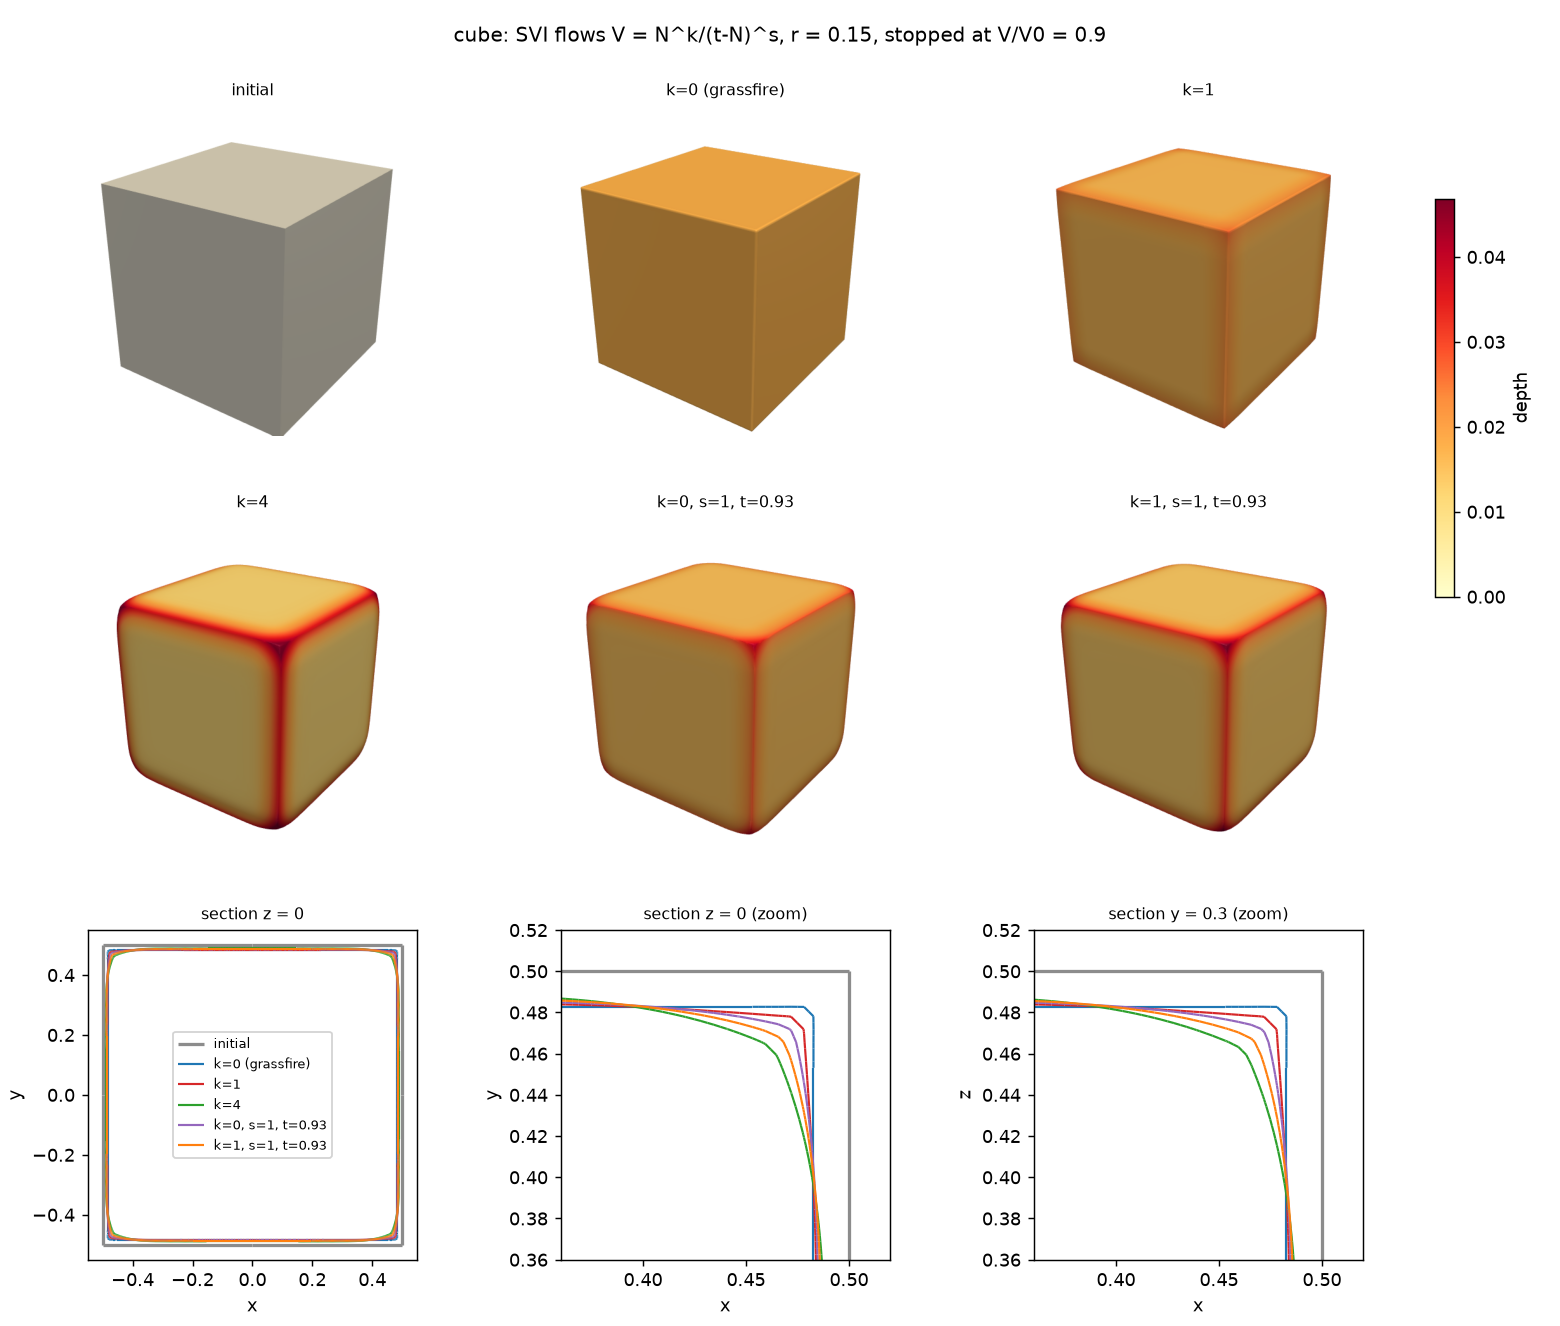
\includegraphics[width=\textwidth]{figures/cube_svi_family.png}
\caption{Cube: the SVI family. Grassfire ($k=0$) produces the inner parallel cube with sharp edges; higher
$k$ and the geometric term ($s=1$) concentrate the erosion at edges and corners. The rounded edges end in a
kink (a shock of the Hamilton--Jacobi equation, \cref{sec:linear}).}\label{fig:cube}
\end{figure}

\begin{figure}[p]
\centering
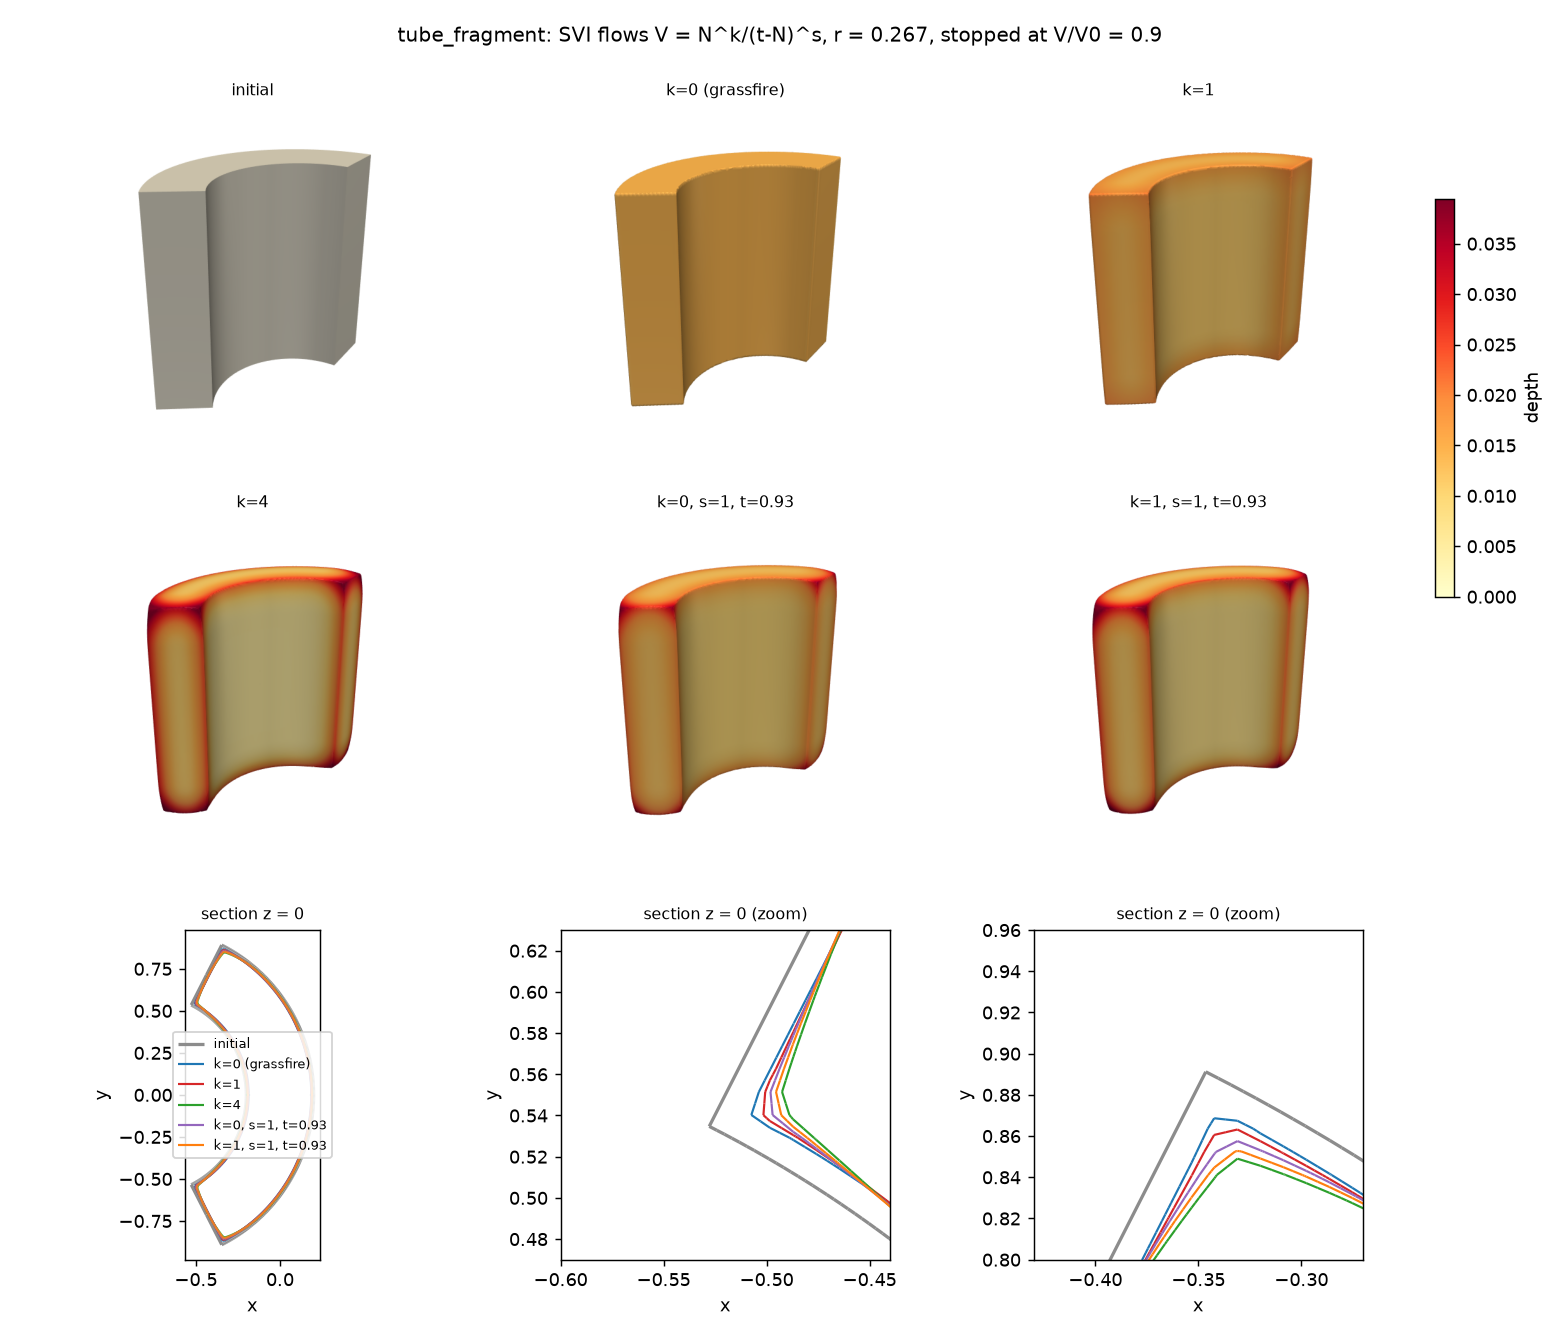
\includegraphics[width=\textwidth]{figures/tube_fragment_svi_family.png}
\caption{Tube fragment: the SVI family. The concave inner (medullary) surface has $\N<\frac12$ and erodes
slowly; the break edges, where the cut faces meet the outer surface, erode fastest.}\label{fig:tube}
\end{figure}

\begin{figure}[p]
\centering
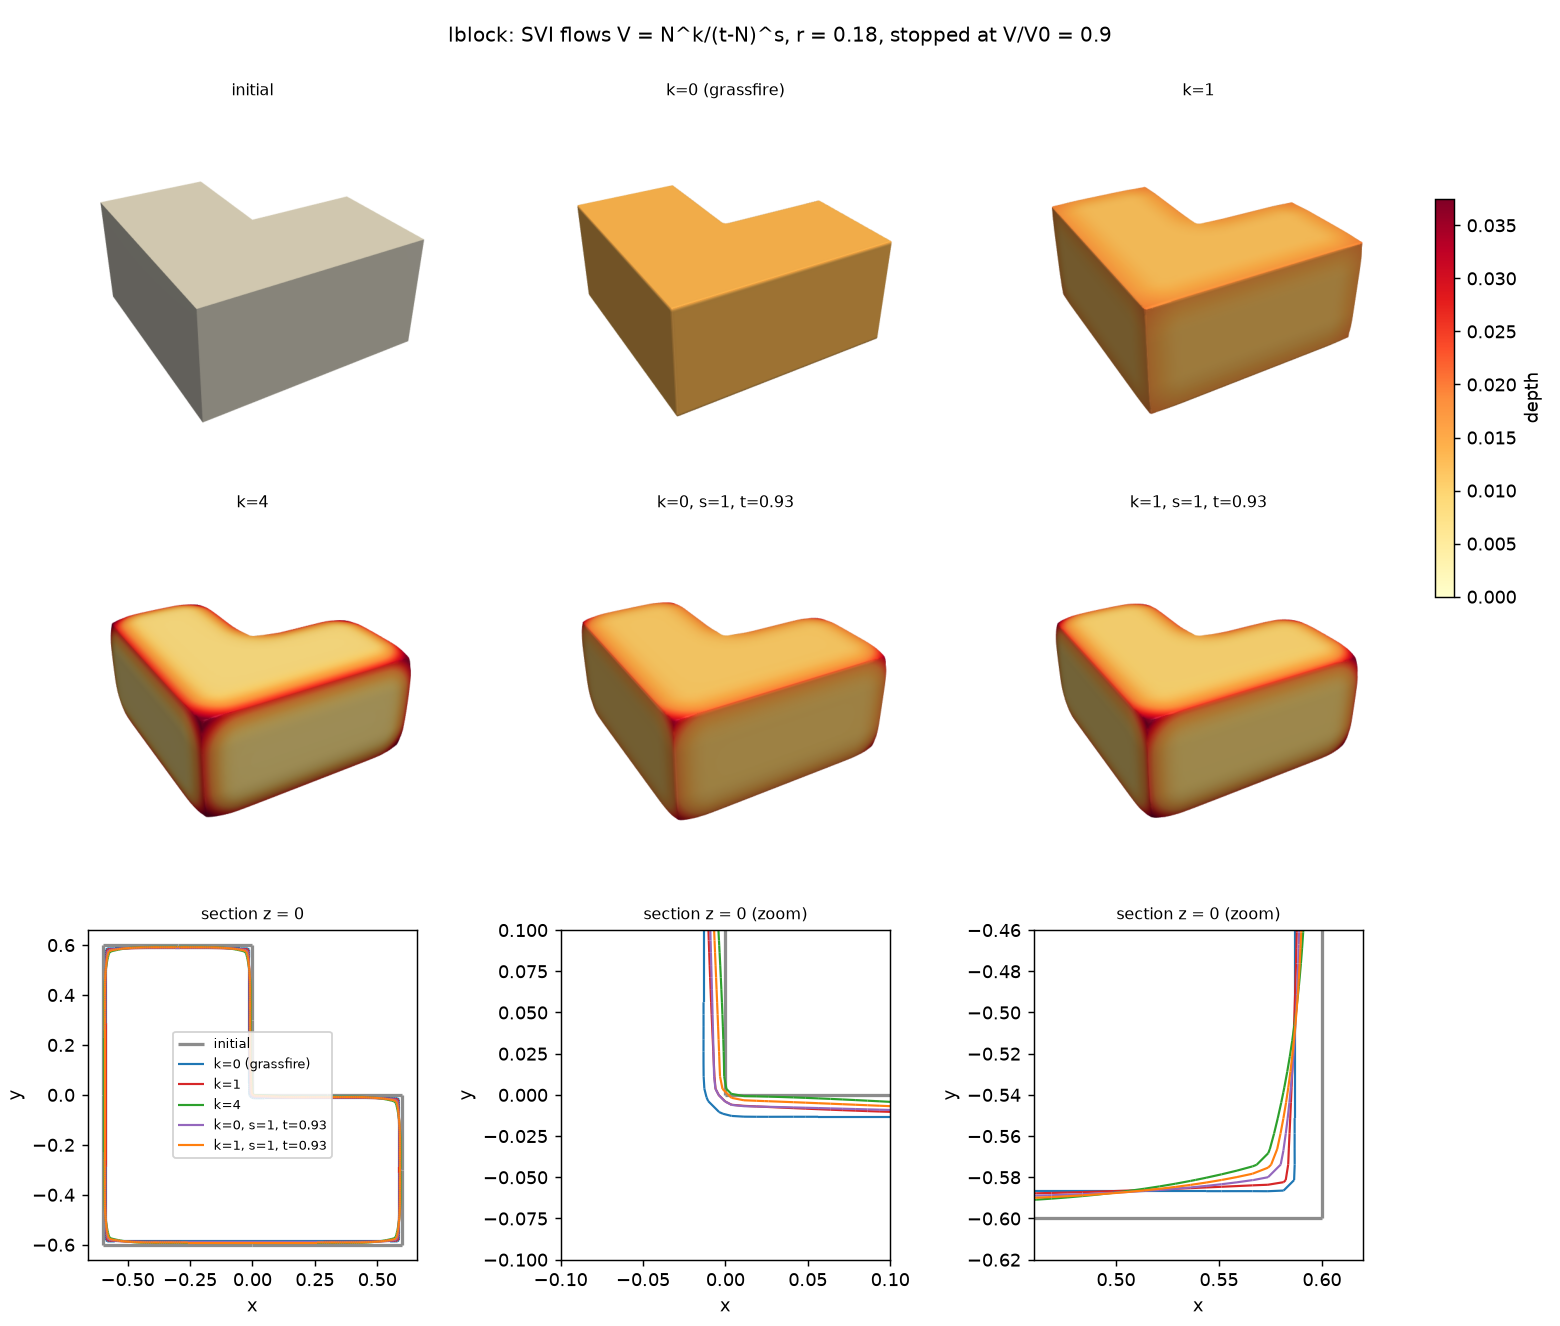
\includegraphics[width=\textwidth]{figures/lblock_svi_family.png}
\caption{L-block: the re-entrant edge ($\N=\frac14$) is protected; with $k=4$ it is almost untouched.}
\label{fig:lblock}
\end{figure}

\begin{figure}[p]
\centering
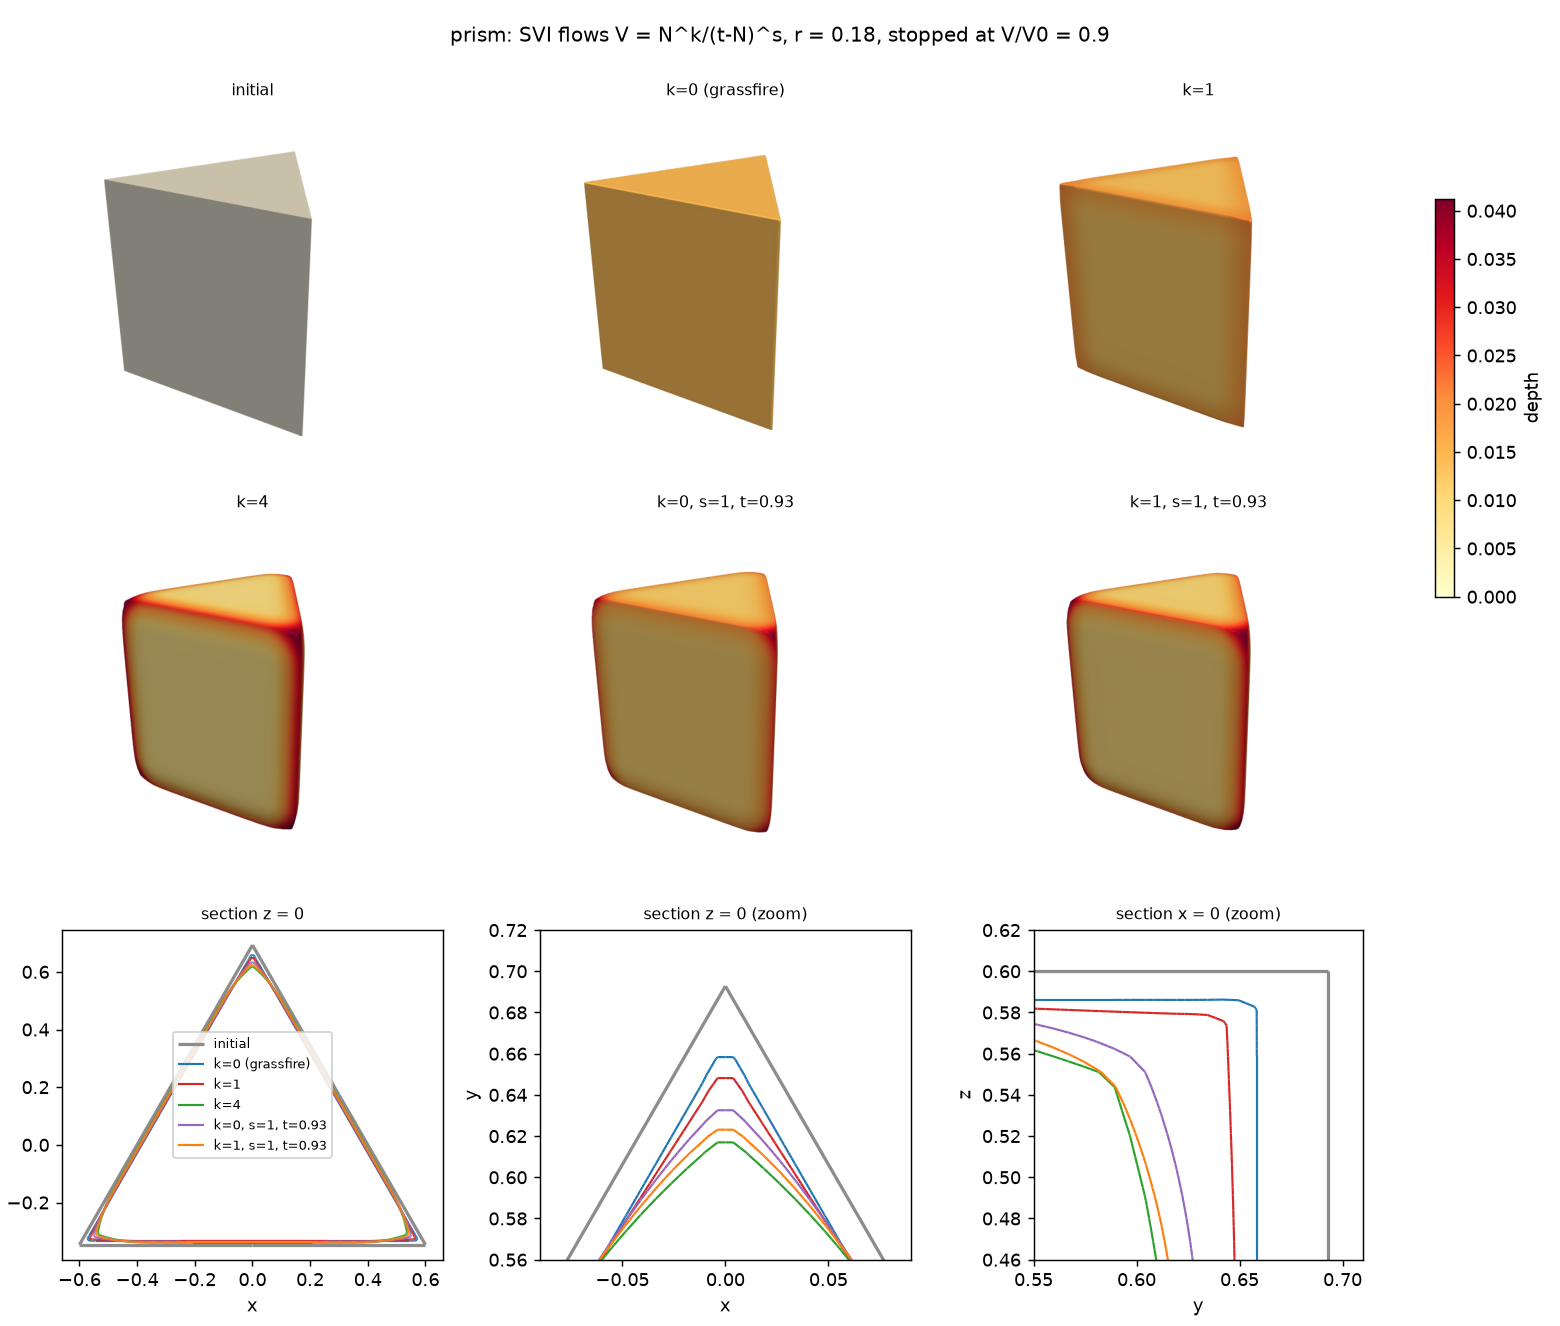
\includegraphics[width=\textwidth]{figures/prism_svi_family.png}
\caption{Triangular prism ($60^\circ$ edges, $\N=5/6$; corners $\N=11/12$).}\label{fig:prism}
\end{figure}

\begin{figure}[p]
\centering
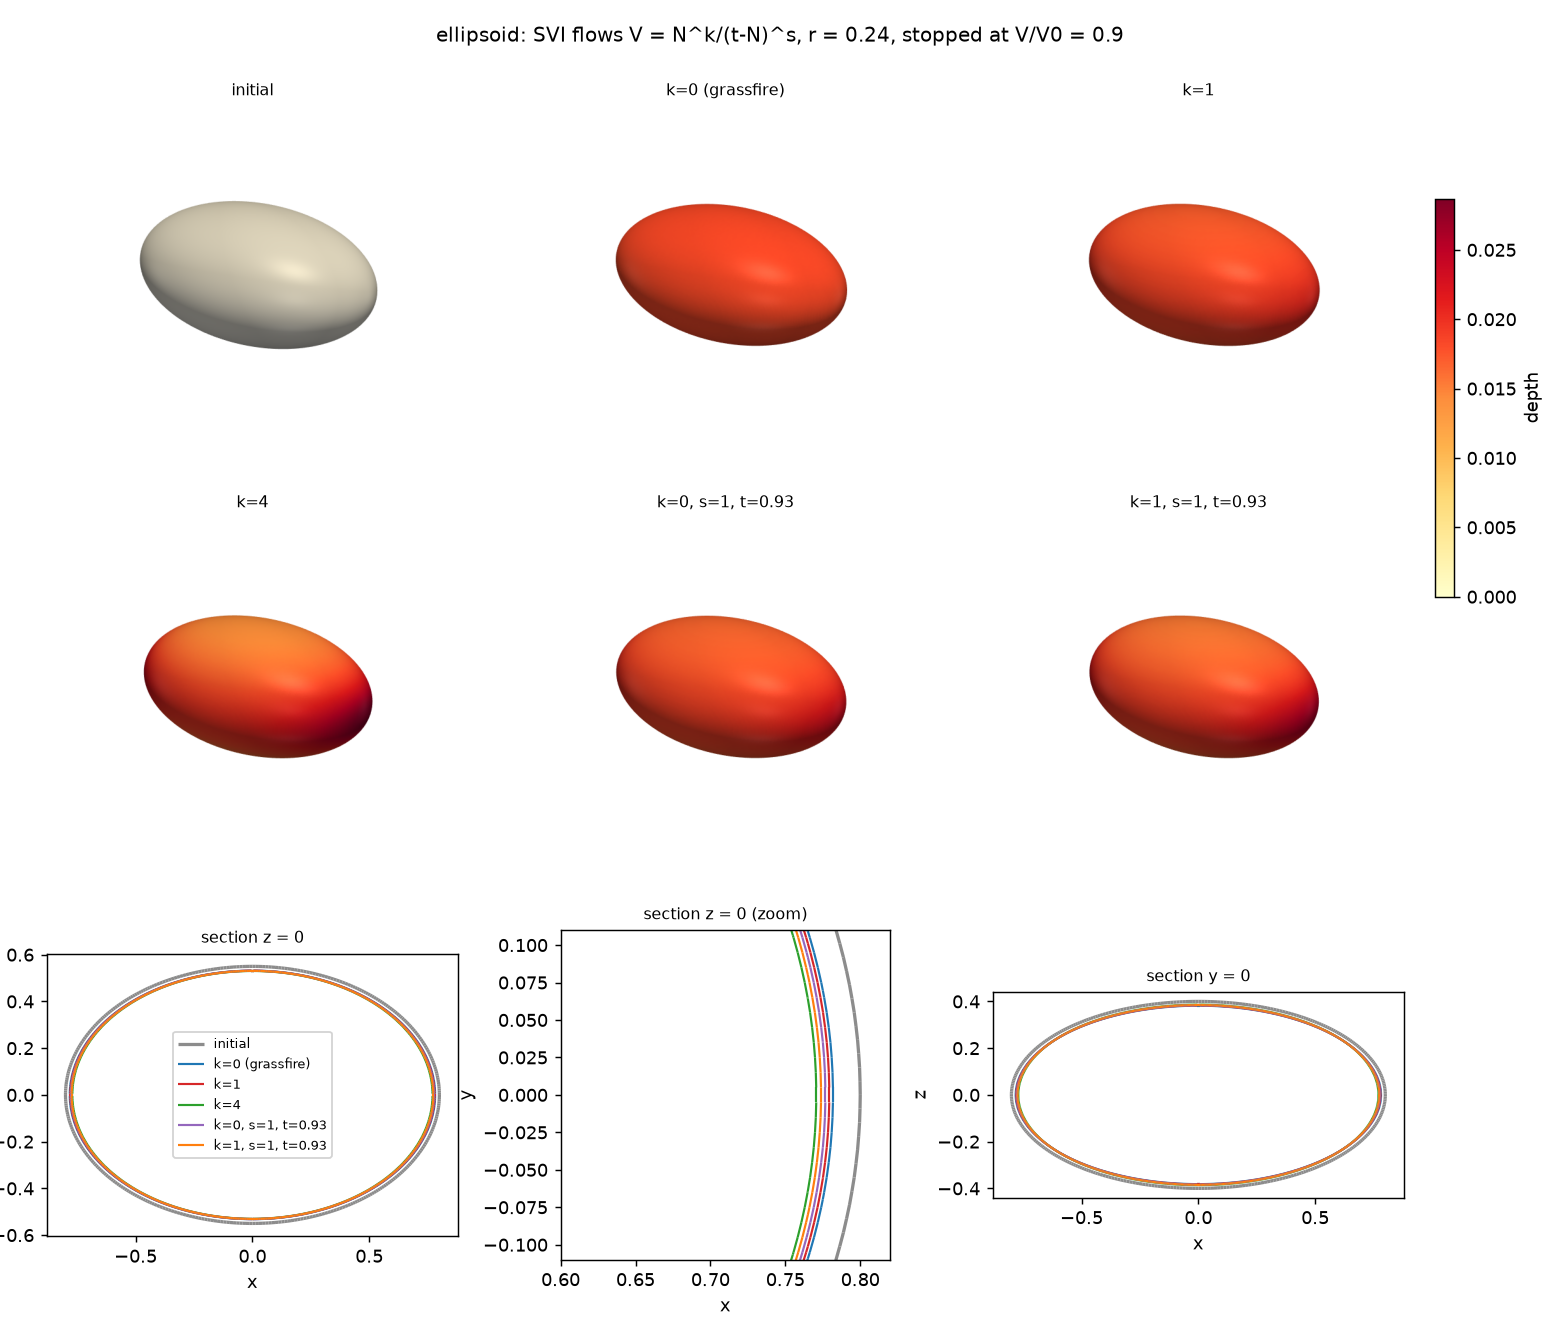
\includegraphics[width=\textwidth]{figures/ellipsoid_svi_family.png}
\caption{Ellipsoid: for a smooth convex body all SVI laws are close to grassfire; larger $k$ and $s=1$
erode the tips of the long axis more.}\label{fig:ellipsoid}
\end{figure}

\begin{figure}[p]
\centering
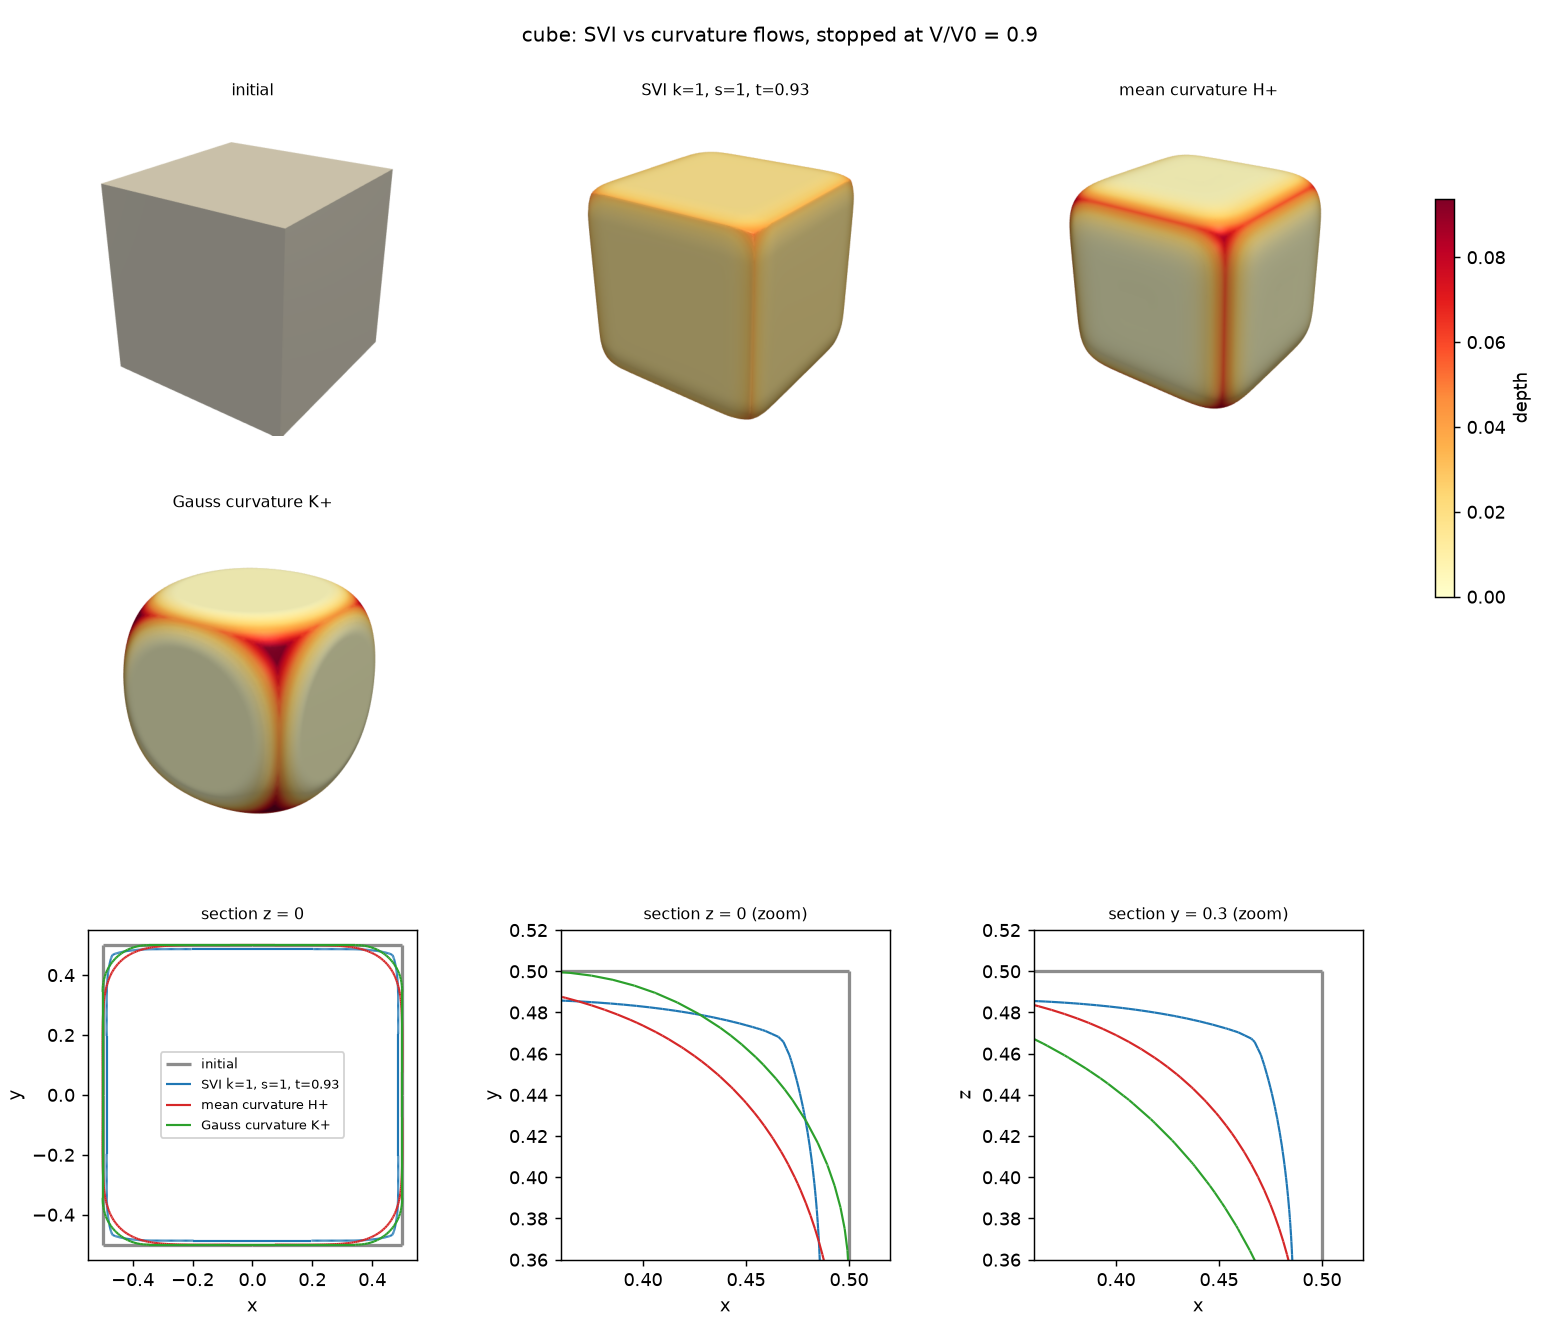
\includegraphics[width=\textwidth]{figures/cube_comparison.png}
\caption{Cube: SVI flow versus curvature flows, all stopped at $90\%$ volume. Under curvature flows the
flat faces do not move at all and the whole volume loss comes from the edges (mean curvature) or only from
the corners (Gauss curvature), producing much larger and rounder bevels.}\label{fig:cubecmp}
\end{figure}

\begin{figure}[p]
\centering
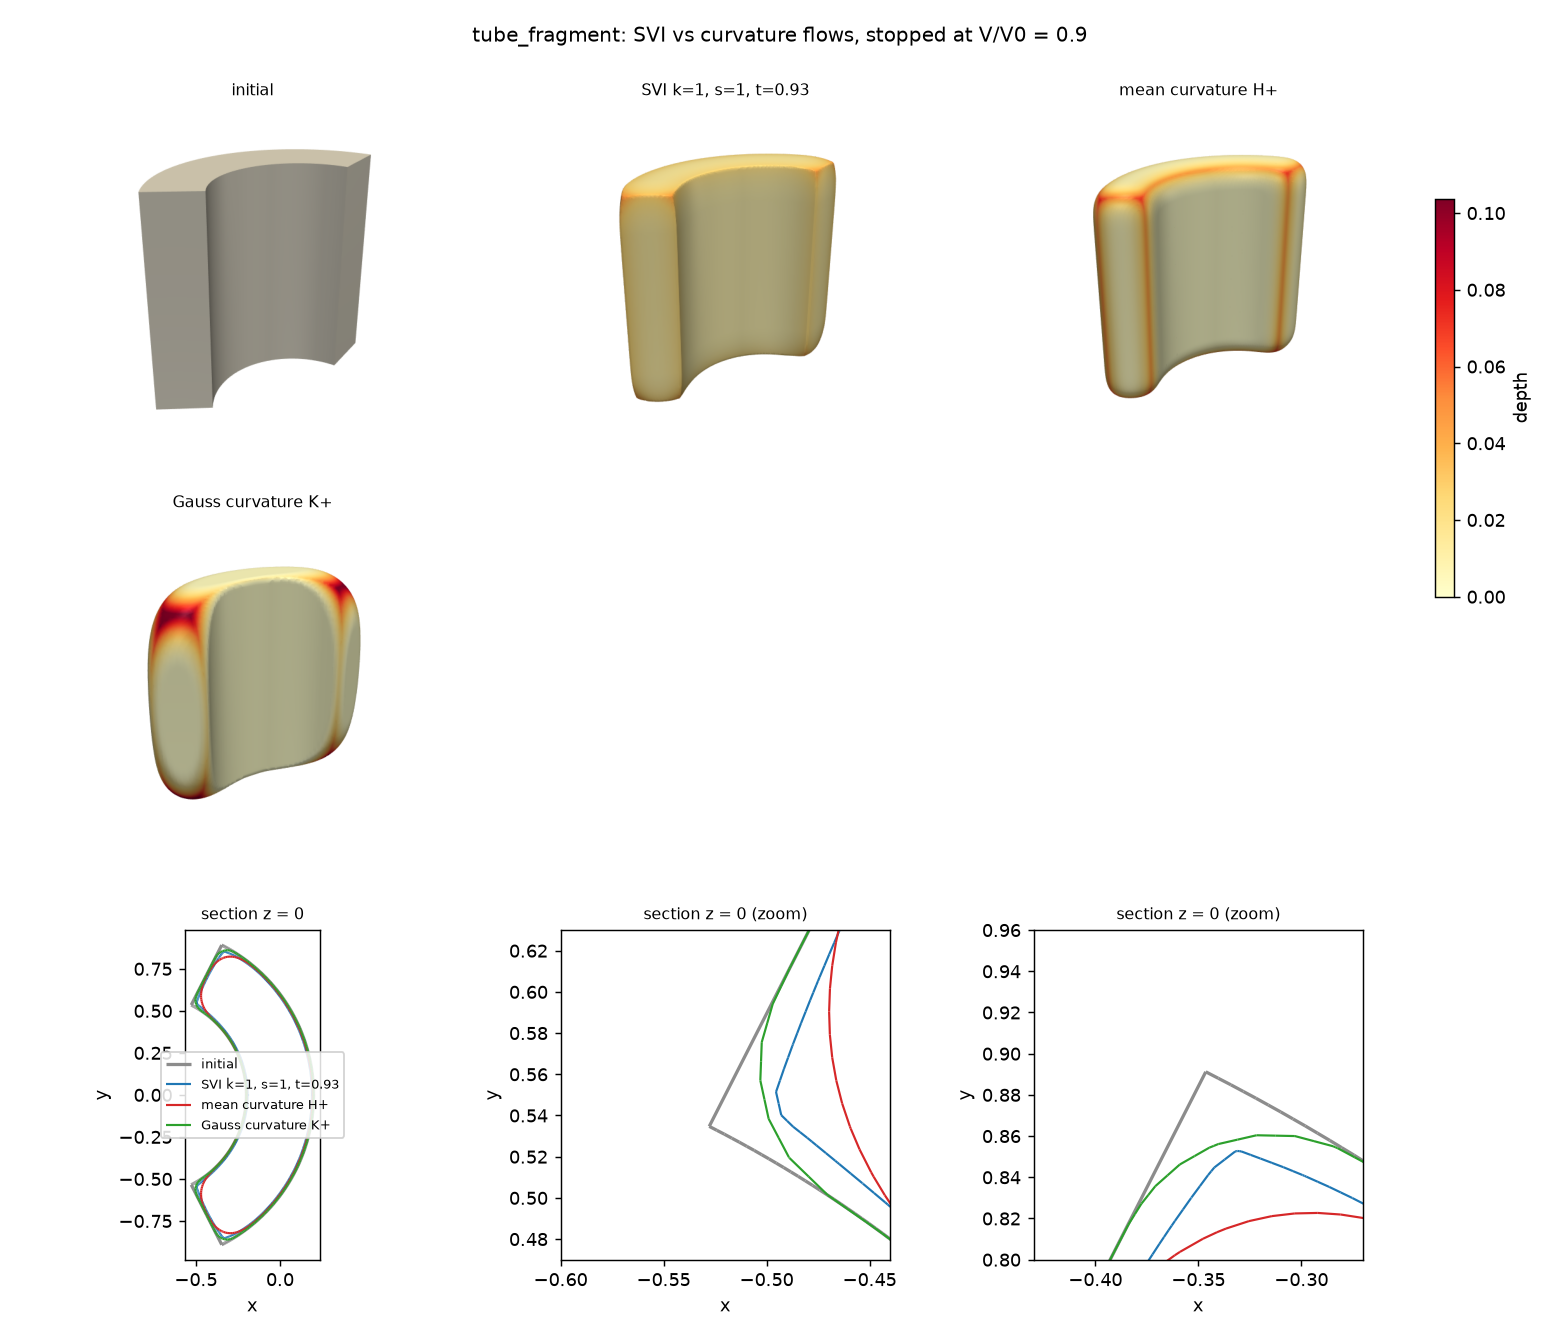
\includegraphics[width=\textwidth]{figures/tube_fragment_comparison.png}
\caption{Tube fragment: SVI flow versus curvature flows.}\label{fig:tubecmp}
\end{figure}

\begin{figure}[p]
\centering
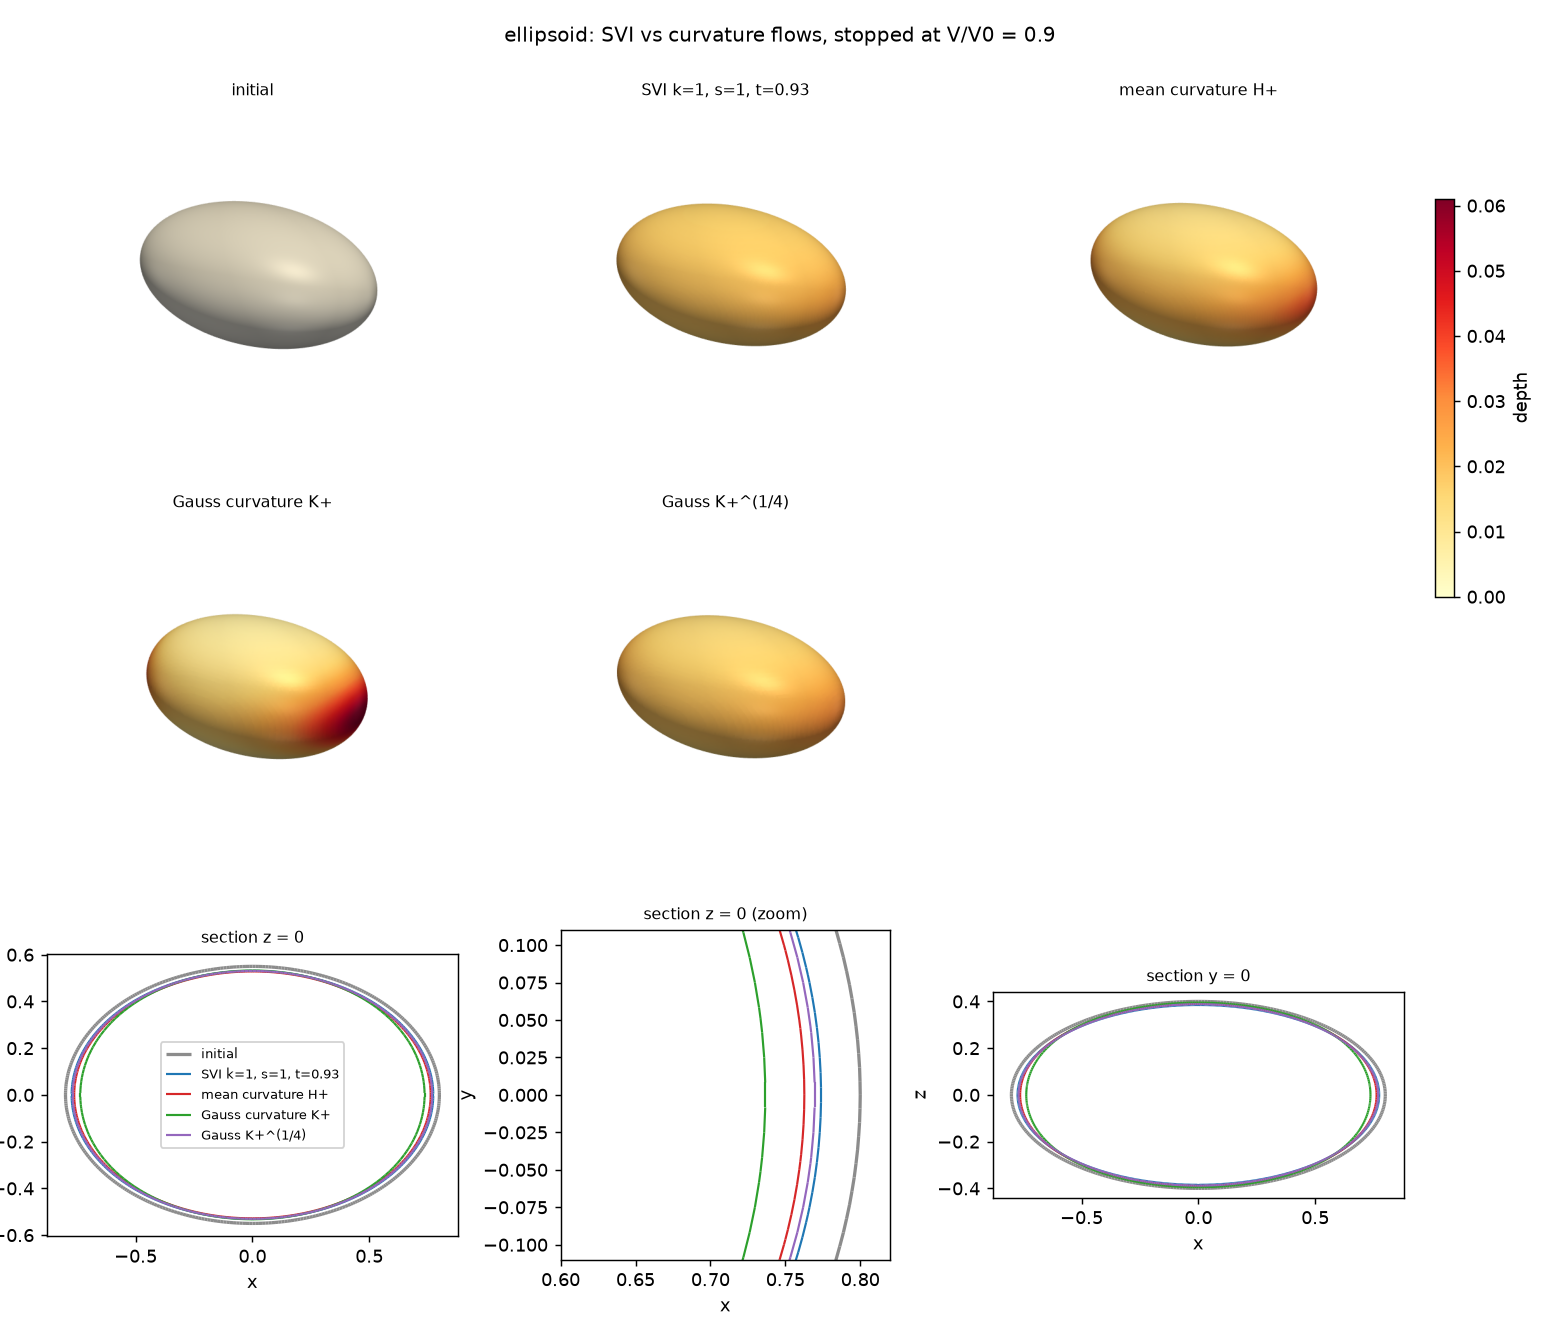
\includegraphics[width=\textwidth]{figures/ellipsoid_comparison.png}
\caption{Ellipsoid: SVI flow versus curvature flows (including the affine flow $K^{1/4}$).}
\label{fig:ellcmp}
\end{figure}

\begin{table}[p]
\centering\footnotesize
\begin{tabular}{llcccc}
\toprule
solid & law & steps & mean depth & max depth & wall [s] \\
\midrule
cube & k=0 (grassfire) & 6 & 0.0172 & 0.0174 & 4.6 \\
cube & k=1 & 9 & 0.0173 & 0.0269 & 1.5 \\
cube & k=4 & 24 & 0.0172 & 0.0541 & 2.5 \\
cube & k=0, s=1, t=0.93 & 20 & 0.0172 & 0.0406 & 2.3 \\
cube & k=1, s=1, t=0.93 & 25 & 0.0172 & 0.0501 & 3.3 \\
cube & mean curvature H+ & 1214 & 0.0166 & 0.0819 & 29.8 \\
cube & Gauss curvature K+ & 5400 & 0.0169 & 0.1042 & 28.5 \\
\midrule
prism & k=0 (grassfire) & 4 & 0.0139 & 0.0155 & 0.9 \\
prism & k=1 & 6 & 0.0138 & 0.0227 & 0.8 \\
prism & k=4 & 19 & 0.0130 & 0.0507 & 1.7 \\
prism & k=0, s=1, t=0.93 & 21 & 0.0135 & 0.0433 & 2.0 \\
prism & k=1, s=1, t=0.93 & 25 & 0.0132 & 0.0508 & 2.2 \\
prism & mean curvature H+ & 626 & 0.0115 & 0.0750 & 10.9 \\
prism & Gauss curvature K+ & 5307 & 0.0104 & 0.1058 & 19.1 \\
\midrule
ellipsoid & k=0 (grassfire) & 4 & 0.0181 & 0.0182 & 0.9 \\
ellipsoid & k=1 & 5 & 0.0182 & 0.0206 & 0.6 \\
ellipsoid & k=4 & 6 & 0.0182 & 0.0293 & 0.7 \\
ellipsoid & k=0, s=1, t=0.93 & 5 & 0.0182 & 0.0232 & 0.7 \\
ellipsoid & k=1, s=1, t=0.93 & 6 & 0.0182 & 0.0261 & 0.7 \\
ellipsoid & mean curvature H+ & 401 & 0.0183 & 0.0373 & 2.4 \\
ellipsoid & Gauss curvature K+ & 574 & 0.0181 & 0.0633 & 1.8 \\
ellipsoid & Gauss K+\^{}(1/4) & 189 & 0.0183 & 0.0303 & 0.8 \\
\midrule
lblock & k=0 (grassfire) & 4 & 0.0133 & 0.0147 & 0.5 \\
lblock & k=1 & 6 & 0.0133 & 0.0201 & 0.7 \\
lblock & k=4 & 15 & 0.0132 & 0.0435 & 1.2 \\
lblock & k=0, s=1, t=0.93 & 13 & 0.0132 & 0.0350 & 1.0 \\
lblock & k=1, s=1, t=0.93 & 16 & 0.0132 & 0.0412 & 1.4 \\
lblock & mean curvature H+ & 516 & 0.0129 & 0.0661 & 7.2 \\
lblock & Gauss curvature K+ & 5571 & 0.0129 & 0.0875 & 17.3 \\
\midrule
tube fragment & k=0 (grassfire) & 3 & 0.0139 & 0.0155 & 3.2 \\
tube fragment & k=1 & 4 & 0.0138 & 0.0215 & 3.4 \\
tube fragment & k=4 & 11 & 0.0134 & 0.0496 & 3.4 \\
tube fragment & k=0, s=1, t=0.93 & 11 & 0.0137 & 0.0423 & 3.3 \\
tube fragment & k=1, s=1, t=0.93 & 14 & 0.0135 & 0.0525 & 3.7 \\
tube fragment & mean curvature H+ & 297 & 0.0122 & 0.0759 & 12.1 \\
tube fragment & Gauss curvature K+ & 3288 & 0.0111 & 0.1227 & 10.4 \\
\bottomrule
\end{tabular}

\caption{Toy runs to $90\%$ volume: number of time steps, mean and maximal erosion depth (distance of the
eroded surface to the original one), and wall-clock time on the GPU.}\label{tab:toy}
\end{table}

\paragraph{Observations.}
\begin{enumerate}
\item \emph{Exposure versus curvature.} The SVI laws erode every exposed surface, including flat faces
(at the rate $F(\frac12)$), and add extra erosion at edges and corners in proportion to their exposure.
Curvature flows do not move flat faces at all, so to remove $10\%$ of the volume they must cut much
deeper into edges and corners: on the unit cube the maximal erosion depth is $0.082$ (mean curvature)
and $0.104$ (Gauss curvature), against $0.017$ (grassfire) to $0.054$ ($k=4$) for the SVI laws
(\cref{tab:toy}). Concave regions are protected under all laws; under the SVI laws they still erode slowly, with a
rate that decreases with $k$.
\item \emph{Kinks.} Because the SVI flow is first order (\cref{sec:linear}), the sharp initial edges are
not instantly rounded: a bevel forms whose two boundaries are kinks that slowly open. Larger $k$ and the
geometric term give wider bevels and blunter kinks (zoomed sections in
\cref{fig:cube,fig:prism,fig:lblock}). Conversely, re-entrant corners are smoothed immediately (they are
rarefaction fans of the Hamilton--Jacobi equation): grassfire carves a fillet whose radius is the erosion
depth, whereas with $k=4$ the re-entrant corner of the L-block hardly moves (\cref{fig:lblock}). A real abraded fragment presumably has smooth edges; whether the SVI flow
should be combined with a small curvature term, or whether this is a reason to prefer an integral over
radii (draft eq.\ (2.7)), is a modelling question.
\item \emph{Geometric term.} For the same flat-surface speed, $s=1$ concentrates erosion far more strongly
at corners than at edges (\cref{tab:ratios}); with $t$ close to $\max\N$ the corners are cut off within
the first few steps.
\end{enumerate}

%======================================================================
\section{The student's code}
%======================================================================

The folder contained \code{svi\_erosion\_1.py} and \code{svi\_erosion.py} (= \code{svi\_erosion\_2.py},
identical files). I read both and used none of their code, but several of their ideas reappear:
\begin{itemize}
\item \emph{Correct and useful:} the sign convention $\phi_t=Q|\nabla\phi|$ with $\phi<0$ inside; the
Godunov formula \eqref{eq:godunov} (first-order version); evaluating $\N$ for the whole grid by an FFT
convolution with a cached kernel transform; a smoothed occupancy instead of a binary count; shortening the
last step by bisection to hit the target volume; checking $\N$ on a sphere against \eqref{eq:Nsphere}.
\item \emph{Limitations:} (i) the mesh was converted to a binary inside/outside array
(\code{trimesh.contains}, one ray query per node) and then redistanced by fast marching, which places
the interface only to $O(h)$ (a staircase); (ii) speeds were evaluated at nodes, with an $O(h/r)$
difference from interface values, and without velocity extension, so $\phi$ degrades and needs frequent
fast-marching redistancing, which itself moves the interface; (iii) first-order upwind differences and
forward Euler (or RK2) in time with a fixed time step derived from a global speed bound; (iv) the
volume invariant itself is $8$--$15$ times less accurate than with the present discretisation
(\cref{tab:N}, row ``student-like + trilinear'');
(v) NumPy on the CPU over the full grid, with a default limit of $3$M voxels; (vi) it needs
\code{trimesh}, \code{rtree} and \code{scikit-fmm}, which were not installed here. The ``integral'' mode
implements $Q=\int_{r_0}^{r_1}dr/|B_r\cap\Omega|$, which is not the law (2.7) of the draft.
\end{itemize}

%======================================================================
\section{Remarks on the draft}
%======================================================================
\begin{enumerate}
\item Equations (6.1)--(6.2) have the wrong sign for $u<0$ inside (they grow the object).
\item The constant in $\N=\frac12+CHr+O(r^2)$ is $C=3/16$ for $H=(\kappa_1+\kappa_2)/2$
(\cref{sec:model}).
\item Section 6 describes the student's implementation (central differences for $\nabla u$, forward Euler,
SVI recomputed every 10 steps, mesh cleaning with \code{pymeshlab}). Central differences are not a stable
discretisation of a Hamilton--Jacobi equation (they produce the oscillations/``spikes'' mentioned in the
comments); the upwind/Godunov schemes of \cref{sec:time} are the standard remedy. With the present code no
mesh cleaning is needed: the output of marching cubes on a band of a signed distance function is a closed,
consistently oriented, manifold triangulation.
\item The comparison with real tumbled fragments needs a rigid registration of the scans before computing
distances; the \code{distance} command computes vertex-wise distances (mean, RMS, Hausdorff) between
already-aligned meshes.
\end{enumerate}

%======================================================================
\section{Limitations and possible extensions}\label{sec:future}
%======================================================================
\begin{itemize}
\item \emph{Grid size.} The method stores dense arrays, so the resolution is limited by memory ($512^3$ fits
on an 8\,GB GPU). For very large or very fine scans a sparse block structure (with overlap-add FFT
convolutions) would remove this limit.
\item \emph{Thin features.} Features thinner than about $2h$ are lost when the mesh is sampled; the
resolution should resolve the thinnest wall of interest.
\item \emph{Several radii.} An integral over radii (draft eq.\ (2.7)) costs one FFT per quadrature radius
with the present code; it would be a small addition (\code{svi.py}).
\item \emph{Gauss curvature flows} on sharp-edged solids need $\Delta t\sim h^3$; a semi-implicit scheme
(e.g.\ Smereka's stabilisation with an FFT Helmholtz solve) or a monotone scheme would make them practical.
\item \emph{Validation against data.} The natural next step is to erode the pre-tumble scans and compare with
the tumbled scans after registration, optimising $(r,k,s,t)$.
\end{itemize}

\begin{thebibliography}{9}
\bibitem{pottmann07} H.~Pottmann, J.~Wallner, Y.-L.~Yang, Y.-K.~Lai, S.-M.~Hu, Principal curvatures from
the integral invariant viewpoint, \emph{Comput.\ Aided Geom.\ Design} 24 (2007).
\bibitem{slepcev03} D.~Slep\v{c}ev, Approximation schemes for propagation of fronts with nonlocal
velocities and Neumann boundary conditions, \emph{Nonlinear Anal.} 52 (2003).
\bibitem{evansspruck} L.C.~Evans, J.~Spruck, Motion of level sets by mean curvature I, \emph{J.\ Differential
Geom.} 33 (1991).
\bibitem{jiangpeng} G.-S.~Jiang, D.~Peng, Weighted ENO schemes for Hamilton--Jacobi equations, \emph{SIAM
J.\ Sci.\ Comput.} 21 (2000).
\bibitem{peng} D.~Peng, B.~Merriman, S.~Osher, H.~Zhao, M.~Kang, A PDE-based fast local level set method,
\emph{J.\ Comput.\ Phys.} 155 (1999).
\bibitem{min10} C.~Min, On reinitializing level set functions, \emph{J.\ Comput.\ Phys.} 229 (2010).
\end{thebibliography}

\end{document}
